\documentclass[11pt,a4paper]{article}

% ═══════════════════════════════════════════════════════════════════════════════
%  THE HARBOR ECONOMY  —  Paper 4 of the Harbor Volume (L3: the market)
%  House style matched to anchor-protocol-whitepaper.tex + agent-transactions +
%  federated-harbor.  hh-* palette, fancyhdr, TikZ figures in figures/.
% ═══════════════════════════════════════════════════════════════════════════════

% ─── Packages ────────────────────────────────────────────────────────────────
\usepackage[utf8]{inputenc}
\usepackage[T1]{fontenc}
\usepackage{lmodern}
\usepackage{geometry}
\usepackage{amsmath,amssymb,amsthm}
\usepackage{hyperref}
\usepackage{listings}
\usepackage{xcolor}
\usepackage{booktabs}
\usepackage{array}
\usepackage{graphicx}
\usepackage{fancyhdr}
\usepackage{tikz}
\usepackage{float}
\usepackage{caption}
\usepackage{enumitem}

\usetikzlibrary{arrows.meta,positioning,fit,backgrounds,calc,shapes.geometric,%
  shapes.symbols,decorations.pathmorphing,decorations.pathreplacing}

% ─── Geometry ────────────────────────────────────────────────────────────────
\geometry{margin=2.5cm}

% ─── Colors (the hh-* harbor palette, shared across the volume) ───────────────
\definecolor{codebg}{RGB}{248,248,248}
\definecolor{codeframe}{RGB}{200,200,200}
\definecolor{darkgreen}{RGB}{0,100,0}
\definecolor{darkblue}{RGB}{0,50,100}
\definecolor{accent}{RGB}{0,128,128}
\definecolor{hhsand}{HTML}{E9DCC4}
\definecolor{hhsanddeep}{HTML}{D4C5A9}
\definecolor{hhebony}{HTML}{1E1B18}
\definecolor{hhink}{HTML}{2C2A26}
\definecolor{hhcinnabar}{HTML}{CC3D2E}
\definecolor{hhbrass}{HTML}{B08D57}
\definecolor{hhpatina}{HTML}{5C7A6A}
\definecolor{hhpaper}{HTML}{FBF7EE}

% ─── Honest-label key markers (ADR-0045 discipline) ───────────────────────────
% One key, used in the header and everywhere a claim is graded.
\newcommand{\Built}{{\textcolor{hhpatina}{\textbf{\textsf{BUILT}}}}}
\newcommand{\BuiltWeak}{{\textcolor{hhbrass}{\textbf{\textsf{BUILT-WEAK}}}}}
\newcommand{\Designed}{{\textcolor{darkblue}{\textbf{\textsf{DESIGNED}}}}}
\newcommand{\Vision}{{\textcolor{hhcinnabar}{\textbf{\textsf{VISION}}}}}

% Verification-status markers (for the open-problem / status tables).
\newcommand{\Closed}{{\textcolor{hhpatina}{\textbf{\textsf{closed}}}}}
\newcommand{\Partial}{{\textcolor{hhbrass}{\textbf{\textsf{partial}}}}}
\newcommand{\Open}{{\textcolor{hhcinnabar}{\textbf{\textsf{open}}}}}

% ─── Pull-quote sidebar: large quote, left-edge accent stripe. ────────────────
\newcommand{\pullquote}[1]{%
  \par\vspace{6pt}%
  \noindent\begin{tikzpicture}
    \node[draw=none,fill=hhsand!40,line width=0pt,
          inner sep=10pt,text width=\dimexpr\textwidth-30pt\relax,
          align=left] (q) {%
      \sffamily\itshape\large #1%
    };
    \draw[hhcinnabar,line width=2.5pt] (q.north west) -- (q.south west);
  \end{tikzpicture}\par\vspace{6pt}%
}

% ─── Teaching callouts: \keyidea{} and \pitfall{} (the pedagogic idiom) ────────
\newcommand{\keyidea}[1]{%
  \par\vspace{6pt}%
  \noindent\begin{tikzpicture}
    \node[draw=hhpatina,line width=1.2pt,fill=hhpatina!12,rounded corners=3pt,
          inner sep=8pt,text width=\dimexpr\textwidth-24pt\relax,align=left] (k) {%
      \small\textbf{\sffamily\textcolor{hhpatina}{Key idea.}}\enspace #1%
    };
  \end{tikzpicture}\par\vspace{6pt}%
}
\newcommand{\pitfall}[1]{%
  \par\vspace{6pt}%
  \noindent\begin{tikzpicture}
    \node[draw=hhcinnabar,line width=1.2pt,fill=hhcinnabar!8,rounded corners=3pt,
          inner sep=8pt,text width=\dimexpr\textwidth-24pt\relax,align=left] (p) {%
      \small\textbf{\sffamily\textcolor{hhcinnabar}{Pitfall.}}\enspace #1%
    };
  \end{tikzpicture}\par\vspace{6pt}%
}

% ─── Companion-paper / cross-reference box ────────────────────────────────────
\newcommand{\xrefbox}[1]{%
  \vspace{4pt}\noindent\begin{tikzpicture}
  \node[draw=hhebony,thick,fill=hhsand!30,rounded corners=2pt,
        inner sep=8pt,text width=\dimexpr\textwidth-22pt\relax,align=left]{%
    \small #1};
  \end{tikzpicture}\vspace{4pt}%
}

% ─── Exercises environment (the pedagogic block) ──────────────────────────────
\newenvironment{exercises}{%
  \par\vspace{8pt}\noindent
  {\sffamily\bfseries\textcolor{hhebony}{\rule[-1pt]{2.5pt}{11pt}\enspace Exercises}}
  \par\nobreak\vspace{2pt}
  \begin{enumerate}[label=\textbf{E\arabic*.},leftmargin=2.6em,itemsep=2pt,topsep=2pt]
}{%
  \end{enumerate}\vspace{6pt}
}
% star marker for open-problem exercises
\newcommand{\openstar}{{\textcolor{hhcinnabar}{$\bigstar$}}\;}

% ─── Listings Setup ──────────────────────────────────────────────────────────
\lstdefinestyle{pseudocode}{
  backgroundcolor=\color{codebg},
  frame=single,
  rulecolor=\color{codeframe},
  basicstyle=\ttfamily\small,
  keywordstyle=\color{darkblue}\bfseries,
  commentstyle=\color{darkgreen}\itshape,
  stringstyle=\color{accent},
  numbers=left,
  numberstyle=\tiny\color{gray},
  numbersep=8pt,
  breaklines=true,
  showstringspaces=false,
  tabsize=2,
  xleftmargin=15pt,
  xrightmargin=5pt,
  framexleftmargin=15pt,
  captionpos=b
}
\lstset{style=pseudocode}

% ─── Theorem Environments ─────────────────────────────────────────────────────
\theoremstyle{definition}
\newtheorem{definition}{Definition}[section]
\newtheorem{theorem}{Theorem}[section]
\newtheorem{lemma}{Lemma}[section]
\newtheorem{proposition}{Proposition}[section]
\newtheorem{property}{Property}[section]
\newtheorem{corollary}{Corollary}[section]
\newtheorem{conjecture}{Conjecture}[section]

\theoremstyle{remark}
\newtheorem*{remark}{Remark}

% ─── Header/Footer ────────────────────────────────────────────────────────────
\pagestyle{fancy}
\fancyhf{}
\fancyhead[L]{\small\textit{The Harbor Economy}}
\fancyhead[R]{\small\thepage}
\fancyfoot[C]{\small Port Daddy --- Harbor Volume, Paper 4 (L3) --- pre-release}
\renewcommand{\headrulewidth}{0.4pt}
\renewcommand{\footrulewidth}{0pt}

% ─── Title ────────────────────────────────────────────────────────────────────
\title{
  \vspace{-1cm}
  {\Large\textsc{Technical White Paper --- Harbor Volume, Paper 4}}\\[0.5cm]
  \rule{\textwidth}{0.5pt}\\[0.3cm]
  {\LARGE\textbf{The Harbor Economy:}}\\[0.2cm]
  {\Large A Three-Sided Market for Agent Labor,\\
   Settling on One Conserving Bond Ledger}\\[0.3cm]
  \rule{\textwidth}{0.5pt}
}
\author{
  \textbf{Erich Owens}\\[0.2cm]
  Curiositech LLC\\[0.2cm]
  \texttt{engineering@portdaddy.dev}
}
\date{June 2026\\Harbor Volume, Paper 4 of 4 (L3 --- the market)}

% ═══════════════════════════════════════════════════════════════════════════════
\begin{document}

\maketitle
\thispagestyle{empty}

\vspace{0.6cm}

\begin{abstract}\noindent
The first three papers of this volume build a harbor for a \emph{single} operator:
a daemon (Paper~2), a coordination protocol (Paper~2), a legible authority anyone
would pay for today (Paper~1), and the continuity that turns an anonymous
\emph{spawn} into an accountable \emph{person} (Paper~3). This paper is the rung
above all of them --- the only one whose participants are plural and mutually
distrusting. We argue that the harbor economy is a \textbf{three-sided market}:
operators sell labor and fleet-for-hire; agents and fleets are rentable assets;
skills and tools are licensed --- all settling on \emph{one} conserving bond
ledger via float-plan escrow. We present the \textbf{Anchor Protocol proper} (the
cross-harbor capability-transfer ceremony, ADR-0014, moved here from Paper~2's
title-scope), and the federation that lets fleets on machines you do not own trade
without a shared chain: a witness log, an escrow that provably cannot steal, and
revocation gossip with a convergence bound. We carry the volume's heaviest
reconciliations honestly rather than papering over them: the keystone identity ADR
covers a single-operator threat model, \emph{not} the cross-operator adversary this
market is defined by (we name the gap \textbf{ADR-0040b}); ``conservation composes
upward'' is a true functor only within a single unit of account and a $\varphi$-
bounded \emph{lax} functor otherwise; reputation is monotone in honest outcomes but
individually revocable by a propagating tombstone; every folk-theorem incentive-
compatibility claim rests on a grading oracle that must be made strategy-proof or
bonded; and strict conservation is budget balance, so by Myerson--Satterthwaite the
market must sacrifice efficiency. The defensible product is \textbf{hosted trust}
--- a verified ledger, a relay, and a reputation system --- not the commoditized
payment rail.
\end{abstract}

\vspace{0.4cm}
\noindent\textbf{Keywords:} mechanism design, multi-sided markets, incentive
compatibility, reputation systems, capability-based security, cross-chain
settlement, applied category theory, federation, Port Daddy

\vspace{0.4cm}
\noindent\textit{Reading time: approximately 45 minutes end-to-end; about 12
minutes for \S\ref{sec:thesis}--\S\ref{sec:three-sides} alone (the market thesis).
This is Paper~4 of a four-paper volume and is written cold: no prior Port Daddy
knowledge is assumed. It can be read first, but \S\ref{sec:keystone} leans on
Paper~3 (\emph{From Spawn to Person}) for the identity substrate, and the
cryptographic \texttt{auth-chain} it rides on is proven in Paper~2 (\emph{The
Anchor Protocol substrate}).}

\vspace{0.5cm}

% ─── Honest-label key (in the header region, per house style) ─────────────────
\noindent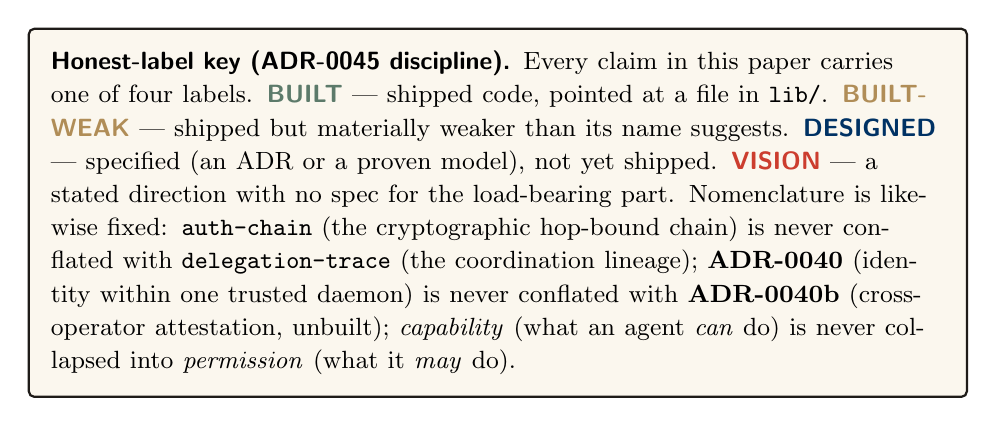
\begin{tikzpicture}
\node[draw=hhebony,thick,fill=hhpaper,rounded corners=2pt,
      inner sep=8pt,text width=\dimexpr\textwidth-22pt\relax,align=left]{%
  \small\textbf{\sffamily Honest-label key (ADR-0045 discipline).}\enspace
  Every claim in this paper carries one of four labels.
  \Built{} --- shipped code, pointed at a file in \texttt{lib/}.
  \BuiltWeak{} --- shipped but materially weaker than its name suggests.
  \Designed{} --- specified (an ADR or a proven model), not yet shipped.
  \Vision{} --- a stated direction with no spec for the load-bearing part.
  Nomenclature is likewise fixed: \texttt{auth-chain} (the cryptographic
  hop-bound chain) is never conflated with \texttt{delegation-trace} (the
  coordination lineage); \textbf{ADR-0040} (identity within one trusted daemon) is
  never conflated with \textbf{ADR-0040b} (cross-operator attestation, unbuilt);
  \emph{capability} (what an agent \emph{can} do) is never collapsed into
  \emph{permission} (what it \emph{may} do).%
};
\end{tikzpicture}

\newpage
\tableofcontents
\newpage

% ═══════════════════════════════════════════════════════════════════════════════
\section{Reader's map}\label{sec:readers-map}
% ═══════════════════════════════════════════════════════════════════════════════

This paper is the top rung of a ladder (Figure~\ref{fig:he-stack-map}). It assumes
the rungs below it and cites the papers that build them. Read it cold if you must,
but it is the fourth paper for a reason: it depends on everything underneath.

% The L0->L3 stack map, viewed from Paper 4 (the L3 market rung).
% Design: one bold title + small-caps whom per rung, one italic content line
% with an honest-state tag; the through-line and dependency moral live in the
% caption, not the canvas.
\providecolor{hhsand}{HTML}{E9DCC4}
\providecolor{hhsanddeep}{HTML}{D8C7A6}
\providecolor{hhebony}{HTML}{121212}
\providecolor{hhink}{HTML}{1B1712}
\providecolor{hhcobalt}{HTML}{003FB8}
\providecolor{hhamber}{HTML}{6B4500}
\providecolor{hhteal}{HTML}{00564C}
\providecolor{hhpaper}{HTML}{FBF7EF}
\providecolor{maydayred}{HTML}{8B0000}

\begin{figure}[H]
\centering
\resizebox{0.92\textwidth}{!}{%
\begin{tikzpicture}[
  font=\small,
  rung/.style={draw=hhebony,thick,rounded corners=3pt,inner sep=7pt,
               minimum width=132mm,minimum height=15mm,align=left,text width=124mm},
  paper/.style={draw=hhink,thick,fill=hhpaper,rounded corners=2pt,inner sep=4pt,
                font=\footnotesize,align=center,text width=22mm},
]

% status tag: cobalt glyph + small-caps grade (the volume's whole vocabulary)
\def\stbuilt{{\footnotesize\textcolor{hhcobalt}{$\blacksquare$}\,\textsc{built}}}
\def\stdesigned{{\footnotesize\textcolor{hhcobalt}{$\square$}\,\textsc{designed}}}

% ─── The four rungs, L0 at the bottom ──────────────────────────────────
\node[rung,fill=hhsand!30] (l0) at (0,0)
  {{\bfseries L0 --- The Daemon (kernel)}\hfill{\footnotesize\textsc{for the machine}}\\[2pt]
   \textit{always-on local truth: ports, claims, sessions, the conserving bond ledger}\hfill\stbuilt};
\node[rung,fill=hhsand!30,above=5mm of l0] (l1)
  {{\bfseries L1 --- Coordination protocol}\hfill{\footnotesize\textsc{for the agents}}\\[2pt]
   \textit{typed conversation, commitments, the hop-bound authorization chain}\hfill\stdesigned};
\node[rung,fill=hhsand!30,above=5mm of l1] (l2)
  {{\bfseries L2 --- Legibility \& authority (the wedge)}\hfill{\footnotesize\textsc{for the operator}}\\[2pt]
   \textit{digest-with-zoom, roadmap-as-truth, adversarial review, the console}\hfill\stbuilt};
\node[rung,fill=hhsand!30,draw=hhcobalt,very thick,above=5mm of l2] (l3)
  {{\bfseries L3 --- Economy \& federation}\hfill{\footnotesize\textsc{for operators, plural \& distrusting}}\\[2pt]
   \textit{cross-harbor capability transfer, float-plan escrow, reputation, federation}\hfill\stdesigned};

% "this paper" flag on L3
\node[anchor=west,font=\bfseries\footnotesize,text=hhcobalt]
  at ([xshift=3mm]l3.east) {$\blacktriangleleft$ this paper};

% companion floors / beams, left column
\node[paper,anchor=east] at ([xshift=-9mm]l0.west) {Floor 1\\\emph{Kernel} \& Beam A \emph{Anchor}};
\node[paper,anchor=east] at ([xshift=-9mm]l2.west) {Floor 2\\\emph{Legible Swarm}};
\node[paper,anchor=east] at ([xshift=-9mm]$(l2.north west)!0.5!(l3.south west)$) {Floor 3\\\emph{Spawn to Person}};
\node[paper,draw=hhcobalt,very thick,anchor=east] at ([xshift=-9mm]l3.west) {\textbf{Floor 4}\\\emph{this}};

\end{tikzpicture}%
}
\caption{Where this paper sits. The L0$\to$L3 substrate stack: each rung serves
a different \emph{whom}, and each announces what it assumes from below. The lower
floors and Beam A climb L0/L1 (kernel, Anchor), L2 (Legible Swarm), and the L3
identity bridge (Spawn to Person); the Harbor Economy is the top floor --- the only
one whose participants are plural and mutually distrusting, and it depends on every
rung below it. It consumes the built bond ledger from L0, the cryptographic
hop-bound authorization chain from L1, and the legible \emph{person} from Floor 3,
and turns them into a market. The volume's spine runs straight up this stack
(Figure~\ref{fig:he-spine-pipeline}): memory becomes a person, registered outcomes
become reputation, and reputation becomes a tradeable asset.}
\label{fig:he-stack-map}
\end{figure}


\begin{table}[H]
\centering
\small
\caption{Where to enter, by who you are.}
\label{tab:readers-map}
\begin{tabular}{@{}p{3.6cm} p{6.2cm} p{4.6cm}@{}}
\toprule
\textbf{If you are\dots} & \textbf{\dots start here} & \textbf{\dots load-bearing artifact} \\
\midrule
A founder asking ``what is the product'' &
  \S\ref{sec:thesis} (thesis) $\to$ \S\ref{sec:hosted-trust} (hosted trust) &
  Fig.~\ref{fig:he-three-sided}; the three claims C1--C3 \\
A mechanism designer &
  \S\ref{sec:three-sides} $\to$ \S\ref{sec:ic} (the formal model) &
  Thm.~\ref{thm:ms}, Fig.~\ref{fig:he-grading-oracle} \\
A cryptographer / distributed-systems reviewer &
  \S\ref{sec:keystone} (the keystone) $\to$ \S\ref{sec:federation} &
  Fig.~\ref{fig:he-keystone-split}, Fig.~\ref{fig:fh-xfer} \\
A category theorist &
  \S\ref{sec:conservation} $\to$ \S\ref{sec:sheaf} &
  Fig.~\ref{fig:he-conservation-functor}, Conj.~\ref{conj:sheaf} \\
A Port Daddy engineer &
  \S\ref{sec:float-plan} (the built floor) $\to$ \S\ref{sec:honest} (status) &
  Table~\ref{tab:honest-state} \\
\bottomrule
\end{tabular}
\end{table}

\noindent\textbf{Reading order within the volume.} Paper~1 (\emph{The Legible
Swarm}, L2 --- the wedge) is the front door. Paper~2 (\emph{The Anchor Protocol
substrate}, L0/L1) is the cryptographic and kernel core. Paper~3 (\emph{From Spawn
to Person}, the L3 identity bridge) supplies the durable identity and the outcome
ledger this paper trades on. \emph{This} paper, Paper~4, is the market that stands
on all three.

% ═══════════════════════════════════════════════════════════════════════════════
\section{The thesis: a market, not a payment rail}\label{sec:thesis}
% ═══════════════════════════════════════════════════════════════════════════════

A solo operator running a swarm of coding agents needs three things --- legibility,
accountability, and safety --- and needs \emph{no cryptography at all}, because she
owns every machine in the harbor. That is the single-player wedge of Paper~1. The
instant two operators trade, the world changes. Alice's frigates touch your
repository. You must now price work done by agents you did not spawn, owned by a
principal you do not trust, using skills you cannot inspect. That is a
\emph{market-design} problem before it is a cryptography problem. Cryptography is
the substrate that makes the ledger unforgeable; it is not the product.

\pullquote{You don't sell crypto --- crypto is the substrate; you sell
\textbf{hosted trust}: a verified ledger, a relay, and a reputation system that
lets mutually-distrustful fleets transact across a boundary they do not share.}

Three claims follow, and the rest of the paper defends each:

\begin{itemize}[leftmargin=1.4em,itemsep=3pt]
  \item \textbf{C1 (three sides).} The harbor economy has three \emph{distinct
    incentive constraints} --- operator-for-hire, asset-rental, skill-licensing
    --- not two. Counting them correctly changes the pricing
    (\S\ref{sec:three-sides}).
  \item \textbf{C2 (one ledger, one escrow object).} All three sides settle on the
    same \textbf{float plan} escrowed in the same bond ledger. Conservation of
    value across every settlement path is the invariant that holds the market
    together, and it is the one thing here that is actually \Built{}
    (\S\ref{sec:float-plan}, \S\ref{sec:conservation}).
  \item \textbf{C3 (hosted trust is the moat).} The defensible asset is the
    verified ledger $+$ relay $+$ reputation, not the settlement rail, which the
    2025--26 agentic-payments stack has already commoditized
    (\S\ref{sec:hosted-trust}).
\end{itemize}

\keyidea{The economy is strictly \emph{additive} on top of the single-player tool.
Because all three market sides settle on the \emph{same} built bond ledger, none
of the economy needs to ship before the wedge does. The discipline ``don't chase
the market early'' is \emph{safe} precisely because the market reuses the kernel
primitive. The harbor comes first; the trade comes when the ships do.}

\subsection{The through-line: why a market needs persons, not spawns}

The whole volume climbs one spine (the vertical arrow in
Figure~\ref{fig:he-stack-map}):
\[
\text{memory} \to \text{checkpoint} \to \text{continuity} \to
\underbrace{\text{a \emph{person}, not a \emph{spawn}}}_{\text{Paper 3}} \to
\text{registered outcomes} \to \text{reputation} \to
\underbrace{\text{a tradeable asset} \to \text{the market}}_{\text{this paper}}.
\]
Sides 2 and 3 of the market --- renting an \emph{asset}, licensing a \emph{good}
--- presuppose that there is a \emph{thing} to rent or sell that cannot be
costlessly cloned. You cannot rent a reputation that any spawn can fork, and you
cannot license a skill whose track record is unverifiable. The canonical
cross-layer sentence, repeated identically in Papers~3 and~4, states the dependency
exactly:

\pullquote{The score is cheap; the substrate it scores over --- witnessed outcomes
on a non-forgeable identity --- is the gate.}

\begin{exercises}
\item Give a one-sentence reason the market cannot ship before reputation does,
  using only the word ``clone.''
\item Side~1 (operator-for-hire) does \emph{not} require durable identity in the
  same way sides 2 and 3 do. Why? (Hint: who is the counterparty, and who bears
  the consequence?)
\item \openstar Construct a market design in which sides 2 and 3 exist
  \emph{without} a non-forgeable identity. Argue informally why every such design
  collapses to a Sybil attack (forward-reference \S\ref{sec:keystone}).
\end{exercises}

% ═══════════════════════════════════════════════════════════════════════════════
\section{What a ``side'' is, and why there are three}\label{sec:three-sides}
% ═══════════════════════════════════════════════════════════════════════════════

A \textbf{two-sided market} (\textbf{Rochet \& Tirole}~\cite{rochet2003}, the
foundational reference: \emph{a platform is two-sided when the allocation of the
total price across the two user groups --- not just its level --- affects
transaction volume}) is the canonical frame for a marketplace: buyers on one side,
sellers on the other, the platform tuning who is subsidized to ignite cross-side
network effects. The naïve reading of the harbor economy is two-sided: a
\emph{requester} posts work, a \emph{worker agent} does it.

But ``two-sided'' undercounts. The operational test~\cite{rochet2006} is: how many
distinct, privately-informed parties must the platform individually rationalize into
participating? In a mature harbor there are three, because \emph{the same agent can
be three economically different things} (Figure~\ref{fig:he-three-sided}).

% Reader question: how does Bob's choice change the seller's exposure?
% The chapter's refactor example, not three abstract risk rails.
% Alternative purchases, not three cumulative charges or paid flows.
% Conservation and reputation subject keys remain in the surrounding prose.
\begin{table}[htbp]
\centering
\begingroup
\pdfiglabelfamily\small
\renewcommand{\arraystretch}{1.2}
\begin{tabularx}{\linewidth}{@{}>{\raggedright\arraybackslash}p{.29\linewidth}@{\hspace{1em}}>{\raggedright\arraybackslash}p{.20\linewidth}@{\hspace{1em}}>{\raggedright\arraybackslash}X@{}}
\toprule
\textbf{Bob buys} & \textbf{Payment} & \textbf{Seller's exposure} \\
\midrule
Work from Alice's three-agent fleet & 400 cr bounty & Alice posts 60 cr per agent; 180 cr in sub-bonds. \\
\addlinespace
An afternoon with Alice's specialist & 90 cr rent & Poor work lowers the specialist's reputation---Alice's asset. \\
\addlinespace
Carol's lint-and-type skill & 0.5 cr per file & Carol's fee is released only on successful settlement. \\
\bottomrule
\end{tabularx}
\endgroup
\caption{One refactor, three alternative purchases. Rental and licensing are designed, not shipped; all three use the same escrow. [illustrative]}
\label{tab:he-three-purchases}
\label{fig:he-three-sided}
\end{table}


\begin{enumerate}[leftmargin=1.6em,itemsep=4pt]
  \item \textbf{Operator-for-hire (labor).} An operator who runs a fleet can sell
    its labor to \emph{another} operator. The operator is now a firm taking
    work-for-hire, with margin $=$ bounty $-\,\Sigma(\text{slashed sub-bonds})\,-$
    ledger fee. Its private information is whether its fleet can deliver. It
    internalizes its fleet's risk --- exactly the property that makes a firm
    accountable for its employees.
  \item \textbf{Agent/fleet as rentable asset (capital).} An operator who owns a
    well-reputed specialist can \emph{rent it out}. Now the asset-owner, the
    task-poster, and the worker are three different parties with three different
    incentives. The owner's private information is the agent's true quality; its
    exposure is reputational.
  \item \textbf{Skill/tool as licensed good (IP).} A skill can be \emph{licensed}
    into someone else's float plan --- metered or per-use --- without the licensor
    doing any task work. The licensor's private information is the skill's quality,
    which the buyer cannot inspect before purchase.
\end{enumerate}

These are three \emph{incentive constraints}, not three UI tabs. If the asset owner
is always the task poster, side~2 collapses into side~1; the design discipline is
to count sides by constraints. The harbor has three because \emph{capability} (an
agent) and \emph{competence} (a skill) become separable, tradeable goods once
identity is durable.

\pitfall{Two-sided-market theory's central result is that the \emph{price
structure} --- who subsidizes whom --- is the lever, not the price level. Mis-count
the sides and you mis-structure the subsidy: you charge the side you should be
\emph{paying} to show up. \S\ref{sec:cold-start} returns to this for cold start.}

The framing is not idiosyncratic. The most recent academic treatment of AI labor
markets, \textbf{Chiu, Zhang \& van der Schaar}~(2025)~\cite{chiu2025} (\emph{a
formal model of a three-sided agent labor market}), models exactly agents,
employers, and a reputation system --- confirming that ``reputation system as a
third side'' is the natural structure once agents compete for paid work.

\subsection{The mandatory honesty rider}

The canonical statement of the market's shape carries a rider that must never be
dropped:

\pullquote{The harbor economy is a three-sided market \emph{by design}; two-sided
until reputation ships (ADR-0049 / ADR-0040b). The third side \emph{is} the
tradeable-person terminus of Paper~3.}

Today there is no reputation implementation in \texttt{lib/}; ADR-0048 lists it as
a gated phase. So sides 2 and 3 are \Designed{}, not shipped. What \emph{is} shipped
is the escrow $+$ conservation floor they will sit on. We do not overclaim the
market.

\subsection*{The category-theory caveat: not ``one structure, three decorations''}

It is tempting to call the three sides ``three decorations of one category'': all
ride one float-plan escrow, so they share the same conservation object. That is
true \emph{at the conservation object}. It is false at the \emph{identity object}.
Each side keys reputation on a different entity --- the \textbf{principal} for
labor, the \textbf{asset owner} for rental, the \textbf{content hash} (a specific
skill version) for licensing. Three different ``what reputation keys on'' means
three partial functors into the ledger that \emph{disagree on the identity object}
(the dashed-red band in Figure~\ref{fig:he-three-sided}). The honest claim is:
\emph{isomorphic at the conservation object, non-isomorphic at the identity
object}. Asserting full isomorphism without that qualifier is the decorative-analogy
failure (\S\ref{sec:conservation}).

\begin{exercises}
\item State the operational test for ``how many sides'' in one sentence, then apply
  it to a ride-share platform: how many sides, and why?
\item Side~3 (skill licensing) keys reputation on a \emph{content hash}, not a
  person. What breaks when a licensor ships v2 of a skill? (Hint:
  \S\ref{sec:gaps}, skill versioning.)
\item \openstar A buyer reads a three-axis reputation vector
  $(\text{accuracy},\text{aesthetics},\text{efficiency})$. Specify a disclosure
  rule that lets the buyer weight the axes \emph{without} re-introducing a single
  Goodhart target. Argue why every fixed scalar collapse re-creates the bandit
  framing the design rejects.
\end{exercises}

% ═══════════════════════════════════════════════════════════════════════════════
\section{The float plan: the built floor}\label{sec:float-plan}
% ═══════════════════════════════════════════════════════════════════════════════

Every side settles on one object: the \textbf{float plan}.

\begin{definition}[Float plan]\label{def:float-plan}
A \emph{float plan} (\textbf{ADR-0014}, \texttt{docs/adr/0014-the-anchor-pro\-to\-col.md})
is a signed declaration of intent: a task, a set of \emph{machine-checkable}
acceptance criteria, a compute budget, and a credit bounty. It is the atom all
three market sides escrow against.
\end{definition}

The escrow handshake is a three-step \texttt{ed25519} ceremony
(Figure~\ref{fig:he-float-plan}): the requester signs the float plan; the daemon
opens a SQLite \texttt{EXCLUSIVE} transaction, debits the requester's wallet, and
moves bounty plus bond into an escrow row; the daemon then signs
$\{anchor\_id, plan\_hash\}$, proving to the worker that funds are locked
\emph{before any work runs}. This is the heart of ``no-spawn-without-bond.''

% Figure IV.3 --- atomicity shown as synchronized state traces on a commit rail.
%
% Reader question: at what instant does a worker become admissible to run --
% a signed plan, an attempted debit, or something else?
% Claim: the wallet debit and the escrow-row write happen at the same
% serialized commit; the worker only starts later, once it has verified that
% committed row exists.
% Evidence: Protocol~escrow (prot:escrow), the three numbered steps, and
% Design Invariant conservation (prop:conservation).
% Must distinguish: the commit instant (wallet+escrow, atomic) from the
% worker's own later transition (gated on a signed check), and both from the
% abort branch, where none of the three traces move.
% Grammar chosen: swimlane Gantt over a commit rail (three lanes, one spine)
% -- the reader question is squarely "what overlaps in time, what order comes
% out" (SKILL.md grammar table), and the ceremony is already three actors
% over one clock. Grammar rejected: a three-step actor sequence diagram (the
% atlas' first-choice) would show messages, not the fact that two traces
% change in the SAME transaction while the third lags -- exactly what this
% page argues.
% Five-second test: a reader can point to the one vertical rule where wallet
% and escrow both jump, and see the worker jump only later, at its own mark.
\begin{figure}[H]
\centering
\pdfigurehue{pdgold}%
\begin{tikzpicture}[pd figure,x=1cm,y=1cm]
  % ---- the grid ---------------------------------------------------------
  \def\lx{-0.40}   % row-label column (anchor east)
  \def\x0{0}       % lane start
  \def\xe{8.70}    % lane end
  \def\tzero{0.30} \def\tone{2.60} \def\tcommit{5.30}
  \def\tworker{6.30} \def\tclear{8.40}
  % ---- title --------------------------------------------------------------
  \node[pd title,anchor=west] at (\lx,5.30)
    {execution becomes admissible at one committed transition};
  % ---- the commit rail: the figure's subject ----------------------------
  \draw[pd spine] (\tcommit,-1.55) -- (\tcommit,4.30);
  \node[pd tag,anchor=south] at (\tcommit,4.35) {atomic commit boundary};
  % ---- wallet: steps down at commit, neutral ------------------------------
  \node[pd title,anchor=east] at (\lx,3.60) {wallet};
  \draw[pd rule] (\x0,3.85) -- (\tcommit,3.85) -- (\tcommit,3.35) -- (\xe,3.35);
  \node[pd label,anchor=south west] at ({\tcommit+.15},{3.35+.14}) {debited};
  % ---- escrow row: steps up at commit, the settlement concept -------------
  \node[pd title,anchor=east] at (\lx,2.10) {escrow row};
  \draw[pd rule] (\x0,1.85) -- (\tcommit,1.85);
  \draw[pd focus rule,line width=1.4pt] (\tcommit,2.35) -- (\xe,2.35);
  \draw[pd rule] (\tcommit,1.85) -- (\tcommit,2.35);
  \node[pd focus label,anchor=south west] at ({\tcommit+.15},{2.35+.14}) {row exists};
  % ---- worker state: steps up only after its own verification -------------
  \node[pd title,anchor=east] at (\lx,0.60) {worker state};
  \draw[pd rule] (\x0,0.35) -- (\tworker,0.35);
  \draw[pd ready rule,line width=1.4pt] (\tworker,0.85) -- (\xe,0.85);
  \draw[pd rule] (\tworker,0.35) -- (\tworker,0.85);
  \node[pd label,anchor=north west] at (\x0,0.20) {no process};
  \node[pd ready label,anchor=south west] at ({\tworker+.15},{0.85+.14}) {running};
  \draw[pd thin arrow] (\tcommit,2.20) to[out=-45,in=140] (\tworker,0.95);
  \node[pd label,anchor=south west] at ({\tcommit+.25},1.55) {signed row check};
  % ---- the abort branch: a window, not an instant, and nothing moves ------
  \node[pd title,anchor=east] at (\lx,-0.75) {if aborted};
  \draw[pd breach rule] (\tone,-0.75) -- (\tcommit,-0.75);
  \node[pd breach datum] at (\tcommit,-0.75) {};
  \node[pd note,anchor=north east,text width=3.3cm] at ({\tcommit-.15},-1.00)
    {all three traces stay in their prior state};
  % ---- the ceremony's clock -----------------------------------------------
  \draw[pd rule,->] (\x0,-2.15) -- ({\xe+.25},-2.15);
  \foreach \x/\lab in {\tzero/{signed plan},\tone/{transaction begins},
                       \tcommit/{commit},\tclear/{clearance}}{
    \draw[pd tick] (\x,-2.07) -- (\x,-2.23);
    \node[pd label,anchor=north] at (\x,-2.30) {\lab};}
\end{tikzpicture}
\caption{\textbf{No-spawn-without-bond is a synchronized state transition.}
The wallet debit and the escrow-row write happen at the same commit (the gold
spine): both traces jump on the same serialized transaction. Only after that
committed row is observable, once the worker verifies the signed row check,
does worker state move from nonexistent to running (green) -- strictly later,
never earlier. In the abort window before the commit, no trace moves: the
invariant lives at the transition, not at a component or a message label. [internal]}
\label{fig:he-float-plan}
\end{figure}


\subsection{The bond ledger conserves value (this is built)}

The single most load-bearing primitive --- and the one that is \emph{actually}
\Built{} --- is \textbf{\texttt{lib/bonds.ts}} (\emph{bond escrow for agent
spawning: debit a project wallet into an escrow row before spawn; refund on clean
exit; slash on breach, splitting the slash between the wallet and a commons pool}).
It guards two invariants:

\begin{property}[Conservation]\label{prop:conservation}
$\text{wallet} + \text{escrow} + \text{commons} = \text{supply}$, always. Every
debit has a matching credit. This is verified across ten thousand random operation
traces by \texttt{tests/unit/bonds-conser\-va\-tion-pro\-perty.test.js} --- a real
property test, not an aspiration. (\Built{})
\end{property}

\begin{property}[No-spawn-without-bond]\label{prop:nospawn}
A process enters the \texttt{running} state only if a bond was escrowed against its
agent id. (\BuiltWeak{}: \texttt{lib/bonds.ts} enforces escrow-first, but the
runtime \texttt{running}-state check is documented as a Phase-2 item in
\texttt{lib/actors.ts}, so today the gate is caller-discipline, not runtime-
enforced.)
\end{property}

\keyidea{Conservation is the mathematical glue of a three-sided market. Whatever
happens --- success, partial credit, slash, lease, license --- no value is created
or destroyed; it only moves between wallet, escrow, and commons. A three-sided
market with three settlement paths is coherent \emph{only if it cannot leak}. Port
Daddy already enforces this for the labor side; the contribution of
\S\ref{sec:conservation} is to show the same invariant extends to the rental and
licensing sides \emph{without modification} and \emph{without a second ledger}.}

\subsection{Settlement: four terminal states bound to an oracle}

Settlement reads an \textbf{oracle} (\emph{a trusted source of ground truth the
agent cannot author --- a passing test id, a merged SHA, a satisfied Arbiter
check}) over the acceptance criteria and lands in one of four states.

\begin{table}[H]
\centering
\small
\caption{The four terminal settlement states. Closure binds to an oracle, not to a
free-text ``Result:'' note --- the same Goodhart-resistant discipline ADR-0041
(\texttt{lib/commitments.ts}) imposes: \emph{the agent picks the work; the daemon
derives the grade}.}
\label{tab:settlement}
\begin{tabular}{@{}l p{6.6cm} p{4.4cm}@{}}
\toprule
\textbf{State} & \textbf{Flow of funds} & \textbf{Reputation effect} \\
\midrule
\textbf{Success}  & escrow $\to$ worker (bond refund) $+$ bounty $\to$ worker &
  $+1$ completion \\
\textbf{Partial}  & pro-rata bond $\to$ worker by completed evidence-chain
  fraction; remainder $\to$ salvage fund & salvage recorded \\
\textbf{Sabotage} & bond $\to$ reconstruction commons (100\% slash) &
  failure recorded; ban on threshold \\
\textbf{Dispute}  & escrow $\to$ arbitration hold; 2-of-3 multi-oracle
  (automated / evidence / human) & none until resolved \\
\bottomrule
\end{tabular}
\end{table}

\begin{exercises}
\item Trace the flow of funds for a \textbf{Partial} settlement where the worker
  completed 40\% of the evidence chain. Confirm Property~\ref{prop:conservation}
  holds across the split.
\item Why does closure bind to an oracle rather than a self-reported note? Name the
  attack a free-text ``Result:'' note enables.
\item \openstar The four states assume the acceptance criteria were \emph{right}.
  Design a \emph{float-plan amendment} protocol for the common case where the
  criteria themselves turn out wrong mid-flight (re-sign by both parties, escrow
  top-up/refund delta), preserving Property~\ref{prop:conservation}. (Gap, \S\ref{sec:gaps}.)
\end{exercises}

% ═══════════════════════════════════════════════════════════════════════════════
\section{Three sides on one escrow}\label{sec:three-on-one}
% ═══════════════════════════════════════════════════════════════════════════════

The novel construction is that the rental and licensing sides ride the \emph{same}
float-plan escrow, so conservation holds globally without a second ledger.

\paragraph{Operator-for-hire (labor).} The operator is the requester's
counterparty. It \emph{sub-escrows} a bond for each fleet agent it dispatches
(\texttt{lib/bonds.ts} is already per-agent). Its profit is
$\text{bounty} - \Sigma(\text{slashed sub-bonds}) - \text{ledger\_fee}$. The
operator internalizes its fleet's risk.

\paragraph{Asset rental (capital).} The lease fee is a line item in the float plan.
By \textbf{incomplete-contracts / property-rights theory}
(\textbf{Grossman \& Hart}~1986~\cite{grossman1986}, \emph{when contracts cannot
specify every contingency, the residual control right should go to the party making
the most important non-contractible investment}), the \emph{renter} must hold the
\emph{runtime} control right --- the ability to sandbox, throttle, or revoke the
leased agent mid-task --- while the \emph{owner} bears the reputational consequence.

\keyidea{This is the cleanest economic argument for the Arbiter's \textbf{jail}
(the L1 tool-allowlist $+$ scoped-FS per agent, \texttt{docs/adr/0048}): the jail
is not just safety hygiene, it is the \emph{residual control right that makes
leasing an agent contractible at all}. Here we must respect the volume's
\emph{capability vs.\ permission} distinction (\S\ref{sec:keystone}): the jail
allocates \emph{capability} (what the leased agent \emph{can} do at runtime). The
deontic layer separately governs \emph{permission} (what it \emph{may} do).
``Able but forbidden'' must stay expressible; the jail bounds ability, not norm.}

\paragraph{Skill licensing (IP).} The per-use fee is released to the licensor
\emph{only on green settlement} (metered $+$ clawback). This is forced by
\textbf{Akerlof}'s \emph{market for lemons} (1970~\cite{akerlof1970}, \emph{when
buyers cannot observe quality, price collapses to the average and good goods exit
the market}): a skill's quality is unobservable before use, so a flat upfront
license drives good skills out. Metering $+$ clawback $+$ a Merkle \emph{portfolio
proof} (the skill's prior settled outcomes, anchored in the evidence chain) restore
the seller's incentive to ship quality.

\begin{exercises}
\item Map each of Grossman--Hart's two parties (residual-control-right holder vs.\
  reputational-consequence bearer) onto the rental side's roles. Which one is the
  Arbiter jail?
\item Show that adding a lease line item and a metered-license line item to a float
  plan cannot violate Property~\ref{prop:conservation}, no matter the amounts.
\item \openstar A skill's portfolio proof for v1 says nothing about v2. Specify a
  \emph{version-binding} for the Merkle portfolio proof so a new version starts
  with a discounted inherited prior --- the newcomer policy, but for code.
\end{exercises}

% ═══════════════════════════════════════════════════════════════════════════════
\section{The keystone the market rests on --- and does not yet have}\label{sec:keystone}
% ═══════════════════════════════════════════════════════════════════════════════

Everything above assumes a counterparty's identity is real. This section confronts
the volume's single \emph{blocking} reconciliation: the identity ADR the whole
market leans on covers a threat model that \emph{excludes the cross-operator
adversary the market is defined by}.

% The keystone split: local non-forgeable identity vs cross-operator attestation.
\providecolor{hhsand}{HTML}{E9DCC4}
\providecolor{hhsanddeep}{HTML}{D8C7A6}
\providecolor{hhebony}{HTML}{121212}
\providecolor{hhcobalt}{HTML}{003FB8}
\providecolor{hhamber}{HTML}{6B4500}
\providecolor{hhteal}{HTML}{00564C}
\providecolor{hhpaper}{HTML}{FBF7EF}
\providecolor{maydayred}{HTML}{8B0000}

\begin{figure}[H]
\centering
\resizebox{0.95\textwidth}{!}{%
\begin{tikzpicture}[
  font=\small,
  harbor/.style={draw=hhebony,thick,fill=hhsand!30,rounded corners=4pt,
                 inner sep=6pt,minimum width=52mm,minimum height=34mm,align=center},
  root/.style={draw=hhink,line width=1.4pt,fill=hhsand!30,rounded corners=2pt,
               inner sep=3pt,font=\scriptsize\bfseries,align=center},
  agent/.style={draw=hhebony,thick,fill=hhpaper,circle,inner sep=1pt,
                minimum size=7mm,font=\scriptsize},
]

% Harbor A
\node[harbor,label={[font=\bfseries\footnotesize]north:Harbor $A$ (Alice owns)}]
  (HA) at (0,0) {};
\node[root] (rA) at ($(HA.center)+(0,9mm)$) {trusted root\\(Alice's daemon)};
\node[agent] (a1) at ($(HA.center)+(-12mm,-7mm)$) {$a_1$};
\node[agent] (a2) at ($(HA.center)+(0,-7mm)$) {$a_2$};
\node[agent] (a3) at ($(HA.center)+(12mm,-7mm)$) {$a_3$};
\foreach \a in {a1,a2,a3} { \draw[->,>=Latex,hhteal,thick] (rA) -- (\a); }

% Harbor B
\node[harbor,label={[font=\bfseries\footnotesize]north:Harbor $B$ (Bob owns)},
  right=46mm of HA] (HB) {};
\node[root] (rB) at ($(HB.center)+(0,9mm)$) {trusted root\\(Bob's daemon)};
\node[agent] (b1) at ($(HB.center)+(-12mm,-7mm)$) {$b_1$};
\node[agent] (b2) at ($(HB.center)+(0,-7mm)$) {$b_2$};
\node[agent] (b3) at ($(HB.center)+(12mm,-7mm)$) {$b_3$};
\foreach \b in {b1,b2,b3} { \draw[->,>=Latex,hhteal,thick] (rB) -- (\b); }

% the keystone the market does NOT have: a missing binding across the boundary.
% drawn in mayday-red with an explicit cross, NOT a tentative blue link.
\node[draw=maydayred,line width=1.6pt,fill=hhpaper,rounded corners=3pt,
      inner sep=4pt,font=\bfseries\scriptsize,text=maydayred,
      text width=36mm,align=center] (gap) at ($(HA.east)!0.5!(HB.west)+(0,4mm)$)
  {\textbf{cross-operator}\\\textbf{attestation}\\ \normalfont\scriptsize
   {\textcolor{hhcobalt}{$\square$}\,\textsc{designed}, not built}\\
   \normalfont\itshape\scriptsize who vouches $b_i$'s keys map to a real distinct
   principal?};
% red dead-ending links from each root toward the boundary, crossed.
\draw[-,line width=1.4pt,maydayred] (HA.east) -- ($(HA.east)!0.42!(HB.west)$);
\draw[-,line width=1.4pt,maydayred] (HB.west) -- ($(HB.west)!0.42!(HA.east)$);
\node[font=\bfseries,text=maydayred,scale=1.6] at ($(HA.east)!0.5!(HB.west)+(0,-9mm)$) {$\times$};


\end{tikzpicture}%
}
\caption{The keystone split. Inside each harbor (teal arrows) a single trusted root
--- the daemon --- vouches for every agent it mints: \textbf{local non-forgeable
identity}, a per-agent identity no agent can edit within one trusted daemon. That is
exactly what a single-operator harbor needs. But the market is defined by
mutually-distrusting operators trading across a boundary neither controls, and that
primitive disclaims the relevant threat model (intra-fleet, not a cross-party PKI,
no hostile-operator defense). The binding across the boundary does not exist --- the
red $\times$ marks it. Binding signing keys across harbors you do not own is a
different, unsolved problem: \textbf{cross-operator attestation}. Across the
boundary the counterparty's daemon \emph{is} the adversary the local threat model
declares out of scope, and the witness log gives log integrity, not identity
binding. It is the highest-leverage unbuilt keystone, and it gates the entire
market thesis.}
\label{fig:he-keystone-split}
\end{figure}


\subsection{ADR-0040 is the keystone --- for Papers 1--3}

\textbf{ADR-0040} (\texttt{docs/adr/0040-non-forgeable-actor-identity.md}) gives a
non-forgeable actor identity \emph{within one trusted daemon}: the daemon is the
only component that can hold state no agent can edit, so it is a trusted root by
construction. For a single-operator harbor (Papers 1--3) this is exactly right and
is correctly named the highest-leverage keystone.

\subsection{But its threat model does not reach L3}\label{sec:0040b}

\pitfall{ADR-0040's \emph{own} threat model is, verbatim, ``a lazy/self-interested
agent in a fleet the operator owns, not a hostile operator,'' and it states ``they
are not a PKI.'' L3 is \emph{defined} by mutually-distrusting operators trading
across a boundary neither controls. You cannot make the single-operator root the
foundation of the cross-operator market without a new ADR. Across the boundary, the
counterparty's daemon \emph{is} the adversary ADR-0040 declares out of scope. The
witness log gives \emph{log integrity}, not \emph{identity binding}: it does not
answer ``who vouches that Harbor~$B$'s \texttt{actor\_id} keys map to a real,
distinct principal?''}

\begin{definition}[The cross-operator attestation problem, ADR-0040b]\label{def:0040b}
\textbf{ADR-0040b} (\emph{unwritten}) is the problem of binding \texttt{actor\_id}
signing keys across harbors you do not own: an actual key-distribution and
attestation story for the cross-operator threat model. \textbf{Status:}
\Designed{}-to-\Vision{}. It is the highest-leverage unbuilt keystone, and it gates
the entire market thesis.
\end{definition}

\keyidea{This paper \emph{stops} describing the federation boundary as one
``neither controls'' while resting on a single trusted root. Either ADR-0040b is
built (a real attestation story), or L3's scope is honestly restated as
``federation among \emph{semi-trusted} operators.'' We take the first horn as the
designed target and flag every claim that depends on it.}

\subsection{The principal above the actor}

The economic counterparty in every trade is the \textbf{principal} (the human or
org owning a fleet), not the agent. Bonds, reputation inheritance, and sanctions
must key on the principal via the \texttt{auth-chain}, or Sybil bond-farming works
by spawning fresh \emph{agents} under one principal (\textbf{Douceur}'s Sybil
attack~\cite{douceur2002}: \emph{free identities defeat any reputation or quorum
system}). Defining the principal as a first-class economic entity is the cleanest
Sybil fix; its cryptographic binding is the identity object specified in Paper~3
and consumed here.

\begin{exercises}
\item In one sentence, state why a reputation system layered on forgeable
  pseudonyms is \emph{no mechanism}, not merely a weak one (cite Douceur).
\item Read the threat-model clause of ADR-0040 quoted above. Name the exact word in
  L3's definition (``mutually-distrusting,'' ``boundary neither controls'') that
  ADR-0040's non-goal contradicts.
\item \openstar Specify a cryptographic binding tying $N$ agents to one principal
  such that spawning fresh agents does not reset the bond floor, and that survives
  into the cross-operator world (where ADR-0040's ``operator-trusted credential
  bypass'' does not). This is ADR-0040b's hard half.
\end{exercises}

% ═══════════════════════════════════════════════════════════════════════════════
\section{Conservation as a functor (and where it is only lax)}\label{sec:conservation}
% ═══════════════════════════════════════════════════════════════════════════════

The economy's single cross-boundary invariant is ``conservation composes upward.''
This section states it precisely --- and demotes it to its proven scope, because the
strong version is false exactly where the open problems live.

% Book-native replacement for fig:he-conservation-functor. Shared Swiss language is preloaded.
\newcommand{\AccConservationDiagram}{%
\begin{tikzpicture}[sg/base,y=-1pt]
  \node[anchor=north west,font=\SGType\bfseries] at (3,0) {one native unit};
  \node[anchor=north east,text=sgTeal] at (318,0) {$-100+80+20=0\ U_A$};
  \SGDocument{accWallet}{(4,27)}{74}{43}{sgViolet!9}{wallet $W$\\$100\ U_A$}
  \SGDocument{accEscrow}{(123,27)}{77}{43}{sgBlue!7}{escrow $E$\\$+80\ U_A$}
  \SGDocument{accCommons}{(238,27)}{77}{43}{sgTeal!8}{commons $C$\\$+20\ U_A$}
  \draw[sg/arrow,draw=sgBlue] (accWallet.east)--node[above,text=sgBlue] {$80\ U_A$}(accEscrow.west);
  \draw[sg/arrow,draw=sgTeal] (accWallet.east)--(96,78)--(96,96)--(276,96)--(276,70);
  \node[anchor=south,text=sgTeal] at (187,92) {$20\ U_A$};
  \node[sg/check,minimum width=307pt,minimum height=25pt,draw=sgTeal,fill=sgTeal!7] at (159,121)
    {$\Delta W=-100\ U_A,\quad\Delta E=+80\ U_A,\quad\Delta C=+20\ U_A$};
  \draw[sgInk,line width=.75pt] (3,143)--(318,143);
  \node[anchor=north west,font=\SGType\bfseries] at (3,154) {quoted conversion};
  \SGDocument{accSource}{(4,181)}{65}{42}{sgViolet!9}{source\\$100\ U_A$}
  \SGDocument{accQuote}{(87,174)}{99}{56}{sgAmber!10}{quote record\\$r_t=0.50\ U_B/U_A$\\source + time $t$}
  \node[sg/check,minimum width=105pt,draw=sgBlue,fill=sgBlue!7] (accGross) at (260,202)
    {quoted gross\\$50\ U_B$};
  \draw[sg/arrow,draw=sgAmber] (accSource.east)--(accQuote.west);
  \draw[sg/arrow,draw=sgBlue] (accQuote.east)--(accGross.west);
  \SGDocument{accNet}{(214,263)}{101}{40}{sgBlue!7}{recipient net\\$47\ U_B$}
  \SGDocument{accFee}{(90,263)}{69}{40}{sgTeal!8}{fee account\\$+1\ U_B$}
  \draw[sg/arrow,draw=sgTeal] (accGross.south)--(260,245)--(124,245)--(124,263);
  \draw[sg/arrow,draw=sgBlue] (accGross.south)--(260,263);
  \node[draw=sgAmber,fill=sgAmber!9,line width=.9pt,minimum width=145pt,minimum height=31pt,align=center] at (245,329)
    {$50-47-1=2\ U_B$\\execution shortfall vs quote};
  \node[anchor=north west,text=sgAmber] at (171,349) {not a literal ledger account};
  \node[anchor=north west,text=sgRed,text width=150pt,align=left] at (4,315)
    {Later exchange rates are not fixed by this quote.};
\end{tikzpicture}}
\begin{figure}[H]
\centering\SGMeasuredFigure{fig-he-conservation-functor}{\AccConservationDiagram}
\caption{Within $U_A$, the illustrated wallet, escrow, and commons deltas sum to zero. A conversion records its rate, time, recipient amount, fee, and the execution shortfall relative to its quote; later rate movement remains an open exposure. [internal; illustrative values]}
\label{fig:he-conservation-functor}
\end{figure}


Each harbor is an object carrying internal structure: a finite category whose
objects are $\{\text{wallet}, \text{escrow}, \text{commons}\}$ and whose morphisms
are the legal money-flows (debit, escrow, slash, settle, refund). The conservation
law (Property~\ref{prop:conservation}) is a \emph{commuting-diagram constraint} in
the sense of \textbf{Spivak's ologs}~\cite{spivak2012} (\emph{an olog is a category
whose objects are types, whose arrows are functional relations, and whose commuting
diagrams are invariants}): every path of settlement morphisms composes to the same
total. The four terminal settlement states are four morphisms out of the escrow
object that must all commute with the conservation functional.

\begin{theorem}[Single-unit federation is a conservative functor]\label{thm:functor}
Restrict to harbors that price bonds in a single, shared unit of account. Then the
federation map $F:\mathbf{Harbor}\to\mathbf{Federation}$, sending each harbor to its
ledger and each cross-harbor transfer to the corresponding federated morphism,
preserves composition: $F(g\circ f)=F(g)\circ F(f)$. Consequently the per-harbor
invariant lifts \emph{exactly} to the federation, with only an in-escrow accounting
term for in-flight bonds. (\Designed{}, proven in the federated-harbor whitepaper as
\texttt{fh-cross-cons}; sketch in Appendix.)
\end{theorem}

\begin{theorem}[Multi-currency federation is at most lax]\label{thm:lax}
If harbors price bonds in heterogeneous units, $F$ is at most a \emph{lax} functor:
conservation is preserved only up to the bounded-escrow slack $\varphi$, via a
coherence 2-cell $F(g\circ f)\overset{\varphi}{\Rightarrow}F(g)\circ F(f)$, and the
coherence conditions are \emph{unproven}. (\Open{}.)
\end{theorem}

\pullquote{The slogan ``conservation composes upward'' is licensed \emph{only} with
its scope rider: a conservation-preserving functor in single-unit-of-account
federation (proven); a $\varphi$-bounded lax functor with unproven coherence in
multi-currency. The headline says ``functor''; honesty requires the footnote say
``lax functor where the units diverge.''}

\subsection{The Myerson--Satterthwaite corner}\label{sec:ms}

Strict conservation (Property~\ref{prop:conservation}) is exactly \emph{budget
balance}. That is not free.

\begin{theorem}[The sacrificed corner]\label{thm:ms}
By \textbf{Myerson--Satterthwaite}~(1983)~\cite{myerson1983} (\emph{no mechanism for
bilateral trade under two-sided private information can be simultaneously efficient,
incentive-compatible, individually-rational, and budget-balanced}), a market that
imposes strict conservation \emph{cannot} also be efficient and individually-
rational and incentive-compatible. The harbor economy keeps budget balance
(conservation), incentive compatibility (settlement is a direct mechanism in the
sense of \textbf{Myerson}~1981~\cite{myerson1981}), and individual rationality
(no party is forced to trade). \emph{The corner it gives up is efficiency}: the
slashing/commons buffer is the budget-balancing wedge that makes the realized
price-of-anarchy strictly worse than first-best.
\end{theorem}

We name this explicitly rather than hide it, and we decline the
d'Aspremont--Gérard-Varet (AGV) escape (which buys budget balance $+$ Bayesian-IC at
the cost of dominant-strategy IC and individual rationality) because IR --- nobody
is forced to enter the harbor --- is non-negotiable for a \emph{voluntary}
federation.

\begin{exercises}
\item State Myerson--Satterthwaite in one sentence, then identify which of its four
  desiderata the harbor sacrifices and why.
\item Theorem~\ref{thm:functor} requires a \emph{single} unit of account. Give a
  concrete two-harbor example where heterogeneous units make $F$ fail to preserve
  composition (the source of Theorem~\ref{thm:lax}'s slack $\varphi$).
\item \openstar Write the coherence 2-cells of the lax functor in
  Theorem~\ref{thm:lax} explicitly and bound them by $\varphi$. Determine whether
  the pentagon/triangle coherence holds.
\end{exercises}

% ═══════════════════════════════════════════════════════════════════════════════
\section{The Anchor Protocol proper: cross-harbor capability transfer}\label{sec:anchor}\label{sec:fh-xfer}
% ═══════════════════════════════════════════════════════════════════════════════

The codebase's ``Anchor Protocol'' (ADR-0014) is the \emph{cross-harbor capability-
transfer ceremony} --- an L3 object, moved here from Paper~2's title-scope, where it
belongs. Paper~2 proves the cryptographic substrate (the \texttt{auth-chain},
ProVerif- and Kani-verified); \emph{this} section is the ceremony that rides it
across a boundary.

% Figure IV.6 --- two coordinated views of the transfer ceremony.
%
% Reader question: what authority changes, which exact messages cross the
%   boundary, and when does Harbor A leave the synchronous path?
% Claim: attenuation narrows C_A twice before B signs C'_B; only the offer and
%   acknowledgement cross the wire, and after the acknowledgement B verifies
%   and delivers locally under sk_B.
% Evidence: the four message names and bound fields in S:fh-xfer-ceremony,
%   plus the chapter's db:write / business-hours attenuation example.
% Must distinguish: authority-set narrowing from message order; local messages
%   from wire messages; synchronous reachback from asynchronous revocation.
% Grammar chosen: an authority-envelope chain over a four-party UML sequence.
%   The two panels share stages but answer different questions. Rejected: one
%   area envelope, because set inclusion is not a continuous quantity.
% Five-second test: name the two wire messages and point to the stage where
%   C'_B becomes destination-local without regaining authority.
\pdfigurehue{pdgold}%
\begin{figure*}[t]
\centering
\begin{tikzpicture}[pd figure,x=1cm,y=1cm]
  \tikzset{
    xfer card/.style={text width=2.65cm,minimum height=2.70cm,
      inner xsep=6pt,inner ysep=6pt,align=center},
    xfer actor/.style={pd artifact,minimum width=2.55cm,minimum height=.72cm,
      inner xsep=6pt,inner ysep=4pt,align=center},
    xfer daemon/.style={pd state,minimum width=2.55cm,minimum height=.72cm,
      inner xsep=6pt,inner ysep=4pt,align=center}
  }

  \node[pd title,anchor=west] at (0,8.50)
    {authority narrows; only two messages cross the wire};

  % Panel A: authority envelope. Set membership, not area, carries the claim.
  \node[pd kind,anchor=west] at (0,7.80) {A\quad Authority envelope};
  \node[pd artifact,xfer card] (capA) at (1.65,6.00)
    {request\\$C_A$\\\texttt{db:write}\\test database};
  \node[pd focus outline,xfer card] (attA) at (5.55,6.00)
    {offer\\A-side attenuation\\\texttt{db:write}\\same resource};
  \node[pd focus state,xfer card] (capB) at (9.45,6.00)
    {acknowledge\\destination card\\\texttt{db:write}\\09:00--17:00};
  \node[pd terminal,pd climax state,xfer card] (localB) at (13.35,6.00)
    {deliver\\destination card\\signed by \texttt{sk\_B}\\verified locally};

  \begin{scope}[on background layer]
    \draw[pd focus arrow] (capA.east) -- (attA.west);
    \draw[pd focus arrow] (attA.east) -- (capB.west);
    \draw[pd focus arrow] (capB.east) -- (localB.west);
  \end{scope}
  \node[pd label,anchor=south] at (3.60,6.20) {att$_A$};
  \node[pd label,anchor=south] at (7.50,6.20) {att$_B$};

  \draw[pd protocol rule] (1.65,4.02) -- (9.45,4.02);
  \draw[pd focus rule] (9.45,4.02) -- (13.35,4.02);
  \node[pd focus datum] at (9.45,4.02) {};
  \node[pd protocol label,anchor=north] at (5.55,3.86)
    {Harbor A participates synchronously};
  \node[pd focus label,anchor=north] at (11.40,3.86)
    {Harbor B verifies locally};

  % Panel B: exact wire protocol. Time advances downward.
  \begin{scope}[yshift=-.60cm]
  \node[pd kind,anchor=west] at (0,3.20) {B\quad Four-message sequence};
  \draw[pd panel] (0.00,2.90) rectangle (7.35,-4.10);
  \draw[pd panel] (7.85,2.90) rectangle (15.20,-4.10);
  \node[pd label,anchor=west] at (.18,2.58) {Harbor $A$ realm};
  \node[pd label,anchor=west] at (8.03,2.58) {Harbor $B$ realm};

  \node[xfer actor] (agentA) at (1.25,1.75) {agent at $A$};
  \node[xfer daemon] (daemonA) at (5.35,1.75) {$D_A$};
  \node[xfer daemon] (daemonB) at (9.85,1.75) {$D_B$};
  \node[xfer actor] (agentB) at (13.95,1.75) {agent at $B$};
  \foreach \x in {1.25,5.35,9.85,13.95}
    {\draw[pd uml lifeline] (\x,1.35) -- (\x,-3.90);}

  \node[pd badge] (m1) at (3.30,.25) {1};
  \node[pd tag,anchor=south] at (3.30,.65)
    {\texttt{xfer\_req}$(C_A,B)$};
  \draw[pd arrow,pd to badge] (1.25,.43) -- (m1);
  \draw[pd arrow,pd from badge] (m1) -- (5.35,.07);

  \node[pd focus badge] (m2) at (7.60,-1.05) {2};
  \node[pd tag,anchor=south,text width=6.7cm,align=center] at (7.60,-.77)
    {\texttt{xfer\_offer}$\langle C_A,\mathrm{att}_A,R_A{}^{(e)}\rangle$};
  \draw[pd protocol arrow,pd to badge] (5.35,-.87) -- (m2);
  \draw[pd protocol arrow,pd from badge] (m2) -- (9.85,-1.23);

  \node[pd focus badge] (m3) at (7.60,-2.35) {3};
  \node[pd tag,anchor=south,text width=6.7cm,align=center] at (7.60,-2.07)
    {\texttt{xfer\_ack}: destination card + epoch root};
  \draw[pd protocol arrow,pd to badge] (9.85,-2.17) -- (m3);
  \draw[pd protocol arrow,pd from badge] (m3) -- (5.35,-2.53);

  \node[pd focus badge] (m4) at (11.90,-3.55) {4};
  \node[pd tag,anchor=south,text width=5.7cm,align=center] at (11.90,-3.27)
    {\texttt{xfer\_deliver}: destination card};
  \draw[pd focus arrow,pd to badge] (9.85,-3.37) -- (m4);
  \draw[pd focus arrow,pd from badge] (m4) -- (13.95,-3.73);
  \end{scope}
\end{tikzpicture}

\caption{Authority narrowing (top) and the four-message ceremony (bottom).
Only the offer and acknowledgement cross the wire; after message 3, Harbor
$B$ verifies locally while later epoch roots carry revocation asynchronously.
[internal]}
\label{fig:fh-xfer}
\end{figure*}


The four-message ceremony (Figure~\ref{fig:fh-xfer}) has one load-bearing liveness
property: after message (3), no further synchronous interaction with Harbor~$A$ is
needed. The transferred card $C_B'$ is verifiable under Harbor~$B$'s key alone, so
federation does not turn every authorization into a synchronous inter-machine round
trip. The epoch root $R_A^{(e)}$ bound into the envelope is the load-bearing
primitive: a revocation issued by $A$ after epoch $e$ invalidates $C_B'$ as soon as
the new root $R_A^{(e+1)}$ reaches the witness log that $B$ audits.

\keyidea{Capability \emph{attenuation} is the safety property here: a transferred
card can only \emph{narrow} authority --- $C_B' = \mathrm{att}_B(\mathrm{att}_A(C_A))$
--- never widen it. This is the cross-boundary form of the attenuation-monotonicity
that the \texttt{auth-chain} guarantees within one harbor (Paper~2). It is what
makes ``rent my agent for an afternoon'' safe to say to a stranger.}

\pitfall{Do not let the federation theorems borrow the Anchor's ``formally
verified'' halo. The \texttt{auth-chain} is mechanized (ProVerif/Kani). The
\emph{federation} theorems (convergence, bounded escrow) are pen-and-paper plus a
TLA\textsuperscript{+} extension; they are \Designed{}, not mechanized. Two
different confidence levels, never blurred.}

\begin{exercises}
\item Why is the ceremony four messages and not two? Identify what message (3)
  buys (Hint: who must counter-sign, and under whose key does $C_B'$ later verify?).
\item Trace what happens to an in-flight $C_B'$ when Alice rotates her signing key
  between messages (3) and a later presentation at $B$. (Gap: cross-boundary key
  rotation, \S\ref{sec:gaps}.)
\item \openstar Specify replay protection across the boundary: is $anchor\_id$ a
  nonce? Does $B$ reject a re-presented message (3)? State the freshness invariant.
\end{exercises}

% ═══════════════════════════════════════════════════════════════════════════════
\section{Federation: trading across machines you don't own}\label{sec:federation}\label{sec:fh-admission}
% ═══════════════════════════════════════════════════════════════════════════════

Federation is where the leaderless distributed canon actually bites. Crucially,
Port Daddy \emph{refuses consensus} here --- the correct reading of the
impossibility landscape.

% Federation topology — the basic gestalt: two harbors, neither root for the other,
% a shared witness log, and a settlement escrow that is structurally bounded.

\providecolor{hhsand}{HTML}{E9DCC4}
\providecolor{hhsanddeep}{HTML}{D8C7A6}
\providecolor{hhebony}{HTML}{121212}
\providecolor{hhink}{HTML}{1B1712}
\providecolor{hhcobalt}{HTML}{003FB8}
\providecolor{hhamber}{HTML}{6B4500}
\providecolor{hhteal}{HTML}{00564C}
\providecolor{hhpaper}{HTML}{FBF7EF}

\begin{figure}[H]
\centering
\resizebox{0.95\textwidth}{!}{%
\begin{tikzpicture}[
  font=\sffamily\small,
  harbor/.style={draw=hhebony,thick,rounded corners=4pt,
                 fill=hhsand!50,inner sep=8pt,minimum width=46mm,
                 minimum height=28mm,align=center},
  harborlbl/.style={draw=hhebony,thick,fill=hhpaper,
                    rounded corners=2pt,font=\sffamily\bfseries\small,
                    inner sep=3pt},
  witness/.style={draw=hhteal,very thick,fill=hhpaper,
                  rounded corners=3pt,inner sep=6pt,
                  minimum width=100mm,minimum height=22mm,align=center,text width=96mm},
  escrow/.style={draw=hhcobalt,thick,fill=hhpaper,
                 rounded corners=3pt,inner sep=6pt,
                 minimum width=46mm,minimum height=16mm,align=center,
                 font=\sffamily\small},
  agentdot/.style={circle,draw=hhebony,fill=hhsanddeep,inner sep=1.5pt},
  edge/.style={->,>=Latex,thick,draw=hhebony},
  gossipedge/.style={->,>=Latex,thick,draw=hhteal,dashed},
  settledge/.style={->,>=Latex,thick,draw=hhcobalt},
]

% ─── Two harbors ───────────────────────────────────────────────────
\node[harbor] (HA) at (0,0) {%
  \textbf{Harbor $A$}\\[2pt]
  \footnotesize Alice's laptop\\
  \footnotesize signing key $\mathit{sk}_A$\\[3pt]
  \begin{tikzpicture}[overlay,remember picture]
  \end{tikzpicture}};
\node[agentdot] at ($(HA.south west)+(8mm,7mm)$) {};
\node[agentdot] at ($(HA.south)+(0,7mm)$) {};
\node[agentdot] at ($(HA.south east)+(-8mm,7mm)$) {};
\node[font=\sffamily\scriptsize\itshape,below=1pt of HA.south,yshift=4mm] {agents under $A$};

\node[harbor,right=44mm of HA] (HB) {%
  \textbf{Harbor $B$}\\[2pt]
  \footnotesize Bob's laptop\\
  \footnotesize signing key $\mathit{sk}_B$\\[3pt]
  };
\node[agentdot] at ($(HB.south west)+(8mm,7mm)$) {};
\node[agentdot] at ($(HB.south)+(0,7mm)$) {};
\node[font=\sffamily\scriptsize\itshape,below=1pt of HB.south,yshift=4mm] {agents under $B$};

% ─── Witness log above ─────────────────────────────────────────────
\node[witness,above=14mm of $(HA)!0.5!(HB)$] (W) {%
  \textbf{Federated Witness Log} \quad \footnotesize (auditor-verifiable, append-only)\\
  \footnotesize epoch roots $R_A^{(e)}, R_B^{(e)}$ \,$\cdot$\, cross-signatures \,$\cdot$\, equivocation evidence};

% ─── Settlement escrow below ───────────────────────────────────────
\node[escrow,below=14mm of $(HA)!0.5!(HB)$] (E) {%
  \textbf{Settlement Escrow}\\[1pt]
  \footnotesize bounded: can refuse, cannot redirect};

% ─── Edges: harbors publish roots up; witness gossips; settlement closes ─
\draw[edge] (HA.north) -- node[font=\sffamily\scriptsize\itshape,above,sloped,xshift=-3mm]{publish $R_A^{(e)}$} (W.south west);
\draw[edge] (HB.north) -- node[font=\sffamily\scriptsize\itshape,above,sloped,xshift=3mm]{publish $R_B^{(e)}$} (W.south east);
\draw[gossipedge] (HA.east) to[bend left=12]
  node[font=\sffamily\scriptsize\itshape,above,midway]{revocation gossip $\Delta$}
  (HB.west);
\draw[settledge] (HA.south) to[bend right=14]
  node[font=\sffamily\scriptsize\itshape,below,sloped,midway]{bond posted at $A$}
  (E.north west);
\draw[settledge] (E.north east) to[bend right=14]
  node[font=\sffamily\scriptsize\itshape,below,sloped,midway]{damage measured at $B$}
  (HB.south);

% ─── Margin annotation: capability transfer ──────────────────────────
\draw[->,>=Latex,thick,draw=hhamber] (HA.east) to[bend left=0]
  node[font=\sffamily\scriptsize\itshape,above,midway,yshift=-1mm,fill=hhpaper,inner sep=1pt]{$\mathsf{xfer}_{A\to B}$ ceremony}
  (HB.west);

\end{tikzpicture}%
}
\caption{The Federated Harbor as a four-element gestalt. Neither harbor is a
root of authority for the other. The witness log above is the shared
correlation device — each harbor publishes its epoch root, and any third party
can audit for equivocation. The escrow below is structurally bounded (it can
refuse to clear, but it cannot redirect funds or equivocate about its
decisions). The amber arrow between the harbors is the cross-harbor capability
transfer ceremony of \S\ref{sec:fh-xfer}; the dashed sage line is the
federated revocation gossip of \S\ref{sec:fh-revocation}. The diagram is
deliberately small: every primitive in the paper attaches to one of these four
elements.}
\label{fig:fh-topology}
\end{figure}


\subsection{No consensus, by design}

\keyidea{A system that \emph{needs} agreement on a global event order across
operators it does not control is dead on arrival, by \textbf{Fischer--Lynch--Paterson}
(1985)~\cite{flp1985} (\emph{no deterministic protocol achieves consensus in an
asynchronous network with even one crash failure}). Federation declines to require
agreement. It requires only (a) append-only per-harbor logs, (b) gossip-bounded
propagation, and (c) \emph{detectable} (not prevented) equivocation. This is a
\textbf{Certificate Transparency} posture~\cite{laurie2014}: you do not prevent a
misbehaving log from lying, you make lying detectable after the fact and expensive
via a slashable bond.}

The convergence and detection bounds smuggle in \emph{partial synchrony}
(\textbf{Dwork--Lynch--Stockmeyer}~1988~\cite{dls1988}, the canonical escape from
FLP): ``gossip every $\Delta$'' \emph{is} an eventual-synchrony assumption, and we
state it as such rather than burying it.

\subsection{Settlement and the cross-chain-deals lineage}\label{sec:fh-settlement}

% Figure IV.8 --- the custody bound is the absence of an extra transition;
% the theorem is tested against its own bypass counterfactual.
%
% Reader question: what exactly does "non-bypassable custody" buy, and what
%   breaks the bound?
% Claim: the bound holds only because the custody ledger exposes exactly one
%   terminal transition; a single extra operator-controlled edge changes the
%   worst case from the agreed fee to the full balance.
% Evidence: Design Invariant (thm:fh-escrow-bound)'s four hypotheses; the two
%   terminal outcomes CLEAR/REFUSE; the extra redirect/second-close edge.
% Must distinguish: the one-edge difference between the two panels from
%   everything else, which is held identical.
% Grammar chosen: two panels on one grid (tpl-before-after.tex idiom), applied
%   to a hypothesis-present/hypothesis-absent counterfactual rather than a
%   time change -- the point is topological (one extra edge), so identical
%   geometry carries it. Grammar rejected: a single diagram with a dashed
%   "optional" edge would blur which panel obeys the theorem's hypothesis; a
%   table would lose the shape of the extra edge.
% Five-second test: which single edge is present in B but not A, and what
%   does it change the worst case to?
\pdfigurehue{pdgold}%
\begin{figure}[H]
\centering
\begin{tikzpicture}[pd figure,x=1cm,y=1cm]
  \def\ax{0.00}   \def\bx{4.95}
  \node[pd title,anchor=west,text width=4.6cm,align=left] at (\ax,2.75) {A. non-bypassable custody};
  \node[pd label,text=pdinkmuted,anchor=north west,text width=5.3cm,align=left] at (\ax,2.20) {one terminal transition};
  \node[pd title,anchor=west,text width=4.6cm,align=left] at (\bx,2.75) {B. operator bypass exists};
  \node[pd label,text=pdinkmuted,anchor=north west,text width=3.9cm,align=left] at (\bx,2.20) {same ceremony, weaker boundary};

  % ---- panel A: funded -> criteria -> Clear / Refuse ---------------------
  \node[pd datum] (fundeda) at (\ax+0.30,0) {};
  \node[pd label,anchor=north] at (\ax+0.30,-0.28) {funded};
  \node[draw=pdinkmuted!70,line width=.9pt,fill=pdpage,diamond,
    minimum width=1.55cm,minimum height=0.95cm,inner sep=0pt,pd label]
    (gatea) at (\ax+1.55,0) {criteria};
  \node[pd focus datum] (cleara) at (\ax+2.85,0.95) {};
  \node[pd datum] (refusea) at (\ax+2.85,-0.95) {};
  \draw[pd arrow] (fundeda) -- (gatea);
  \draw[pd focus arrow] (gatea) -- (cleara);
  \draw[pd arrow] (gatea) -- (refusea);
  \node[pd focus label,anchor=west] at (\ax+3.10,0.95) {\textbf{Clear}};
  \node[pd label,anchor=west] at (\ax+3.10,-0.95) {\textbf{Refuse}};
  \draw[pd focus rule] (\ax+0.05,-1.65) -- (\ax+4.55,-1.65);
  \node[pd focus label,anchor=north west,text width=4.5cm,align=left] at (\ax+0.05,-1.85)
    {worst-case loss $\leq\varphi$};

  % ---- panel B: identical graph, plus one operator-controlled edge -------
  \node[pd datum] (fundedb) at (\bx+0.30,0) {};
  \node[pd label,anchor=north] at (\bx+0.30,-0.28) {funded};
  \node[draw=pdinkmuted!70,line width=.9pt,fill=pdpage,diamond,
    minimum width=1.55cm,minimum height=0.95cm,inner sep=0pt,pd label]
    (gateb) at (\bx+1.55,0) {criteria};
  \node[pd focus datum] (clearb) at (\bx+2.85,0.95) {};
  \node[pd datum] (refuseb) at (\bx+2.85,-0.95) {};
  \node[pd breach datum] (lossb) at (\bx+2.85,-2.55) {};
  \draw[pd arrow] (fundedb) -- (gateb);
  \draw[pd focus arrow] (gateb) -- (clearb);
  \draw[pd arrow] (gateb) -- (refuseb);
  \draw[pd breach arrow,line width=1.25pt] (fundedb) to[out=-75,in=150] (lossb);
  \node[pd focus label,anchor=west] at (\bx+3.10,0.95) {\textbf{Clear}};
  \node[pd label,anchor=west] at (\bx+3.10,-0.95) {\textbf{Refuse}};
  \node[pd breach label,anchor=north,text width=4.2cm,align=center] at (\bx+2.85,-2.95)
    {redirect / second close: full balance exposed};
  \draw[pd breach rule] (\bx+0.05,-4.35) -- (\bx+4.55,-4.35);
  \node[pd breach label,anchor=north west,text width=3.9cm,align=left] at (\bx+0.05,-4.55)
    {worst case $=$ full custody balance};

  \node[pd note,anchor=north west,text width=10.6cm] at (\ax,-6.10)
    {the custody assumption: whitelist, fee cap, one terminal transition are
    the theorem's hypothesis, not decoration};
\end{tikzpicture}
\caption{\textbf{The custody bound is the absence of an extra transition.}
Panel A permits exactly one terminal move from funded custody to \textbf{Clear}
or \textbf{Refuse}: pay the whitelisted beneficiary or return the bond. With a
recipient whitelist and fee cap, worst-case loss is bounded by the agreed fee
$\varphi$. Panel B holds the same ceremony but drops the non-bypassability
hypothesis: one operator-controlled edge reaches redirect or a second close,
and the worst case becomes the full custody balance. Threshold signing
(\S\ref{sec:fh-escrow}) is only one candidate way to make panel A's absence of
that edge structural; the bound holds only when it actually is. [internal]}
\label{fig:fh-settlement}
\end{figure}


The bounded escrow is honest about its trust: it does \emph{not} claim trustless
settlement. The worst-case extraction is the pre-agreed fee $\varphi$ --- \emph{
trusted-but-bounded}, not trustless. This is a deliberate departure from the
hash-timelock baseline (\textbf{Herlihy}~2018~\cite{herlihy2018}, atomic cross-chain
swaps), and the right comparison is the formal model of mutually-distrusting
commerce without a shared chain: \textbf{Herlihy, Liskov \& Shrira}~(2022, \emph{
Cross-Chain Deals and Adversarial Commerce})~\cite{hls2022}. The harbor's bounded
escrow is a ``trusted third party / watchtower'' point in that design space; we
locate it there explicitly rather than reinvent it.

\begin{conjecture}[Trustless cross-harbor settlement]\label{conj:trustless}\label{thm:fh-escrow-bound}
Trustless settlement for \emph{non-fungible, reputation-priced} bonds is impossible
(unlike HTLC for fungible value). Proving or refuting this is the deepest crypto-
economic question in the layer. (\Open{}.)
\end{conjecture}

\subsection{Revocation gossip and the equivocation race}\label{sec:fh-revocation}\label{sec:revocation}

% Figure IV.9 --- staleness is a per-harbor window, not a global clock.
%
% Reader question: how long does a revoked capability stay spendable at each
%   harbor, and does that window ever end?
% Claim: the spendable window is the harbor-specific delay before local
%   synchronization; the issuer has none, and the illustrated execution shows
%   one harbor exposed until Delta and another until 2*Delta.
% Evidence: the worked execution from S:fh-revocation (Alice refuses at 0,
%   B until Delta, C until 2*Delta) under thm:fh-conv's epidemic model.
% Must distinguish: the still-spendable portion of each row (breach, red)
%   from the already-synchronized portion (focus, gold).
% Grammar chosen: swimlane over time, one row per harbor (tpl-swimlane-gantt
%   idiom). Grammar rejected: the v1 figure stacked an area chart, a
%   double-headed exposure arrow, and cream knockout label boxes into one
%   picture -- three devices and a sticker habit the standard forbids; a
%   single smooth curve would assert a continuous quantity the discrete
%   per-harbor bound does not give.
% Five-second test: at time Delta, which harbor can still accept the revoked
%   card, and which already refuses it locally?
\pdfigurehue{pdgold}%
\begin{figure}[H]
\centering
\begin{tikzpicture}[pd figure,x=1cm,y=1cm]
  \def\x0{1.55}   \def\dd{2.72}   \def\rh{0.42}
  \node[pd title,anchor=north west,text width=10.6cm,align=left] at (0,4.45)
    {the spendable window closes when the local authority synchronizes};

  % ---- epoch-root commit points (concrete, auditable) --------------------
  \node[pd focus datum] (e0) at (\x0,3.05) {};
  \node[pd focus datum] (e1) at (\x0+\dd,3.05) {};
  \node[pd focus datum] (e2) at (\x0+2*\dd,3.05) {};
  \draw[pd focus rule] (e0) -- (e2);
  \node[pd focus label,anchor=west,text width=3.5cm,align=left] at (\x0+2*\dd+0.55,3.05)
    {signed epoch roots};

  % ---- row A: Alice refuses immediately, no stale window ------------------
  \node[pd label,anchor=east,text width=1.4cm,align=right] at (\x0-0.20,2.20) {Harbor $A$};
  \draw[pd focus rule] (\x0,2.20-\rh) rectangle (\x0+3*\dd,2.20+\rh);
  \node[pd focus label] at (\x0+1.5*\dd,2.20) {refuses locally};

  % ---- row B: stale until Delta, synchronized after ------------------------
  \node[pd label,anchor=east,text width=1.4cm,align=right] at (\x0-0.20,1.00) {Harbor $B$};
  \draw[pd breach rule] (\x0,1.00-\rh) rectangle (\x0+\dd,1.00+\rh);
  \draw[pd focus rule] (\x0+\dd,1.00-\rh) rectangle (\x0+3*\dd,1.00+\rh);

  % ---- row C: stale until 2*Delta, synchronized after -----------------------
  \node[pd label,anchor=east,text width=1.4cm,align=right] at (\x0-0.20,-0.20) {Harbor $C$};
  \draw[pd breach rule] (\x0,-0.20-\rh) rectangle (\x0+2*\dd,-0.20+\rh);
  \node[pd breach label] at (\x0+0.5*\dd,-0.20) {still spendable};
  \draw[pd focus rule] (\x0+2*\dd,-0.20-\rh) rectangle (\x0+3*\dd,-0.20+\rh);

  % ---- time axis -------------------------------------------------------
  \draw[pd rule,-{Stealth[length=1.8mm,width=1.1mm]}]
    (\x0-0.20,-0.20-\rh-0.55) -- (\x0+3*\dd+0.35,-0.20-\rh-0.55);
  \foreach \k/\lab in {0/$0$,1/$\Delta$,2/$2\Delta$,3/$3\Delta$}
    {\draw[pd tick] (\x0+\k*\dd,-0.20-\rh-0.55) -- (\x0+\k*\dd,-0.20-\rh-0.70);
     \node[pd label,anchor=north] at (\x0+\k*\dd,-0.20-\rh-0.75) {\lab};}
  \node[pd label,anchor=west] at (\x0+3*\dd+0.30,-0.20-\rh-0.55) {time};

  \node[pd note,anchor=north west,text width=9.2cm] at (\x0-0.20,-2.35)
    {gold marks a harbor that has synchronized and refuses the card on its
    own authority; red marks the window in which that card is still spendable
    at that harbor};
\end{tikzpicture}
\caption{\textbf{Revocation propagation is a moving, per-harbor staleness
frontier.} In this illustrated execution Alice (harbor $A$) refuses
immediately; $B$ remains stale until $\Delta$ and $C$ until $2\Delta$. The red
band is exactly where a revoked capability can still be admitted by the named
local authority; the gold epoch-root commits mark synchronization, not a
global clock. Expected $\Theta(\log m)$ dissemination (Theorem~\ref{thm:fh-conv})
requires connected reliable rounds; a partition can extend the red window
without bound and therefore destroys any finite deadline. [internal]}
\label{fig:fh-revocation}
\end{figure}


Federated revocation propagates by anti-entropy gossip
(\textbf{Demers et al.}~1987~\cite{demers1987}) with a cuckoo-filter discipline.
The whitepaper's convergence bound, expected $\Delta(1+\ln m)$ for $m$ harbors,
inherits Demers' \emph{average-case, honest-participant, random-peer} model.

\pitfall{The threat is \emph{adversarial}, not stochastic. An attacker who controls
peer selection or partitions the gossip graph (an \emph{eclipse attack},
\textbf{Heilman et al.}~2015~\cite{heilman2015}) breaks the expected-time guarantee.
The honest statement is: convergence is bounded \emph{under partial synchrony with
honest-majority gossip}, and that is a cryptographic assumption, not a free lemma.}

Detection-after-the-fact deters only if the slashed bond exceeds the value
extractable during the detection window. This is the analogue of the Cleanup Lower
Bound, and we state it as a target:

\begin{conjecture}[Equivocation Lower Bound]\label{conj:eq-bound}\label{thm:fh-conv}
The witness bond must dominate the maximum value spendable against a revoked-but-not-
yet-converged capability across the \emph{worst-case} (not expected) detection
window. Without it, a well-capitalized adversary can rationally equivocate, extract,
and eat the slash. (\Open{}; analogue of the proven Cleanup Lower Bound.)
\end{conjecture}

% Figure IV.10 --- assurance position, not a prose matrix; position is the
% one channel a reader reads accurately (Cleveland-McGill).
%
% Reader question: which threats are mechanized, which are only bounded
%   under a stated model, and which remain open?
% Claim: assurance advances only when a threat acquires a concrete artifact
%   or theorem; most rows are conditional on a named hypothesis, and three
%   remain open.
% Evidence: the seven threat rows and their own evidence phrase (signed
%   card, the Theta(log m) bound, the settlement gate, ...) from S:fh-limitations.
% Must distinguish: OPEN (acknowledged gap) from CONDITIONAL (bound holds
%   under a named hypothesis) from MECHANIZED (artifact exists).
% Grammar chosen: position on one shared axis, seven rows (a banded ledger).
%   Grammar rejected: a checklist table loses the ORDERING claim (rows are
%   not equally mechanized); a decorative shield/lock icon per row asserts
%   security the paper does not claim.
% Five-second test: which single row is closest to MECHANIZED, and which
%   three rows have not moved off OPEN?
\pdfigurehue{pdgold}%
\begin{figure*}[t]
\centering
\begin{tikzpicture}[pd figure,x=1cm,y=1cm]
  \def\lx{1.65}   \def\x0{2.05}   \def\pw{8.35}
  \node[pd title,anchor=north west,text width=10.6cm,align=left] at (0,5.15)
    {assurance advances only when a threat acquires an artifact or theorem};

  \foreach \y/\lab in {3.30/{identity + replay},1.90/{revocation},0.50/{equivocation},
    -0.90/{settlement},-2.30/{cold-start admission},-3.70/{cartel monitoring},
    -5.40/{centralization}}
    {\node[pd label,anchor=east,text width=2.7cm,align=right] at (\lx,\y) {\lab};
     \draw[pd hairline] (\x0,\y) -- (\x0+\pw,\y);}

  % identity + replay -- strongest evidence: chapter's own exemplar
  \draw[pd focus rule,line width=1.2pt] (\x0,3.30) -- (10.05,3.30);
  \node[pd focus datum] at (10.05,3.30) {};
  \node[pd focus label,anchor=south east,text width=3.4cm,align=right] at (10.05,3.48)
    {signed card $+$ epoch root};

  % revocation -- literally the concept; breach hue
  \draw[pd breach rule,line width=1.2pt] (\x0,1.90) -- (7.27,1.90);
  \node[pd breach datum] at (7.27,1.90) {};
  \node[pd breach label,anchor=south east,text width=3.6cm,align=right] at (7.27,2.08)
    {$\Theta(\log m)$ only under reliable rounds};

  % equivocation -- conditional, neutral ink
  \draw[pd rule,line width=1.2pt] (\x0,0.50) -- (6.92,0.50);
  \node[pd datum] at (6.92,0.50) {};
  \node[pd label,anchor=south east,text width=3.4cm,align=right] at (6.92,0.68)
    {proof after roots co-locate};

  % settlement -- wide uncertainty interval, neutral ink (thick = range)
  \draw[pd rule,line width=1.2pt] (\x0,-0.90) -- (6.75,-0.90);
  \draw[pd rule,line width=2.2pt] (5.09,-0.90) -- (7.35,-0.90);
  \node[pd datum] at (6.75,-0.90) {};
  \node[pd label,anchor=south east,text width=3.6cm,align=right] at (6.75,-0.72)
    {bypassable to gated: gate-dependent};

  % cold-start admission -- open, neutral ink
  \draw[pd rule,line width=1.2pt] (\x0,-2.30) -- (4.96,-2.30);
  \node[pd datum] at (4.96,-2.30) {};
  \node[pd label,anchor=south west,text width=4.0cm,align=left] at (2.45,-2.12)
    {thin reputation cannot price a bond};

  % cartel monitoring -- open, neutral ink
  \draw[pd rule,line width=1.2pt] (\x0,-3.70) -- (4.66,-3.70);
  \node[pd datum] at (4.66,-3.70) {};
  \node[pd label,anchor=south west,text width=4.0cm,align=left] at (2.45,-3.52)
    {monitoring game incomplete};

  % centralization -- open, neutral ink; the pushback point (S:fh-limitations)
  \draw[pd rule,line width=1.2pt] (\x0,-5.40) -- (4.22,-5.40);
  \node[pd datum] at (4.22,-5.40) {};
  \node[pd label,anchor=south west,text width=4.0cm,align=left] at (2.45,-5.22)
    {pushback is design discipline, not a bound};

  % ---- assurance-position axis --------------------------------------------
  \draw[pd rule,-{Stealth[length=1.8mm,width=1.1mm]}] (\x0,-6.40) -- (\x0+\pw+0.05,-6.40);
  \foreach \x/\lab in {2.05/OPEN,6.15/CONDITIONAL,10.25/MECHANIZED}
    {\draw[pd tick] (\x,-6.40) -- (\x,-6.55);
     \node[pd label,anchor=north] at (\x,-6.60) {\lab};}
  \node[pd note,anchor=north west,text width=10.2cm] at (0,-7.05)
    {position, not colour, carries the claim: each row advances only when the
    missing artifact or theorem exists};
\end{tikzpicture}
\caption{\textbf{The assurance landscape is uneven and falsifiable.} Position
encodes how far each threat has moved from an acknowledged gap toward a
mechanized artifact. Identity and replay (gold) have the strongest concrete
evidence. Revocation (red) is conditional on connected reliable rounds
(Theorem~\ref{thm:fh-conv}); equivocation and settlement are conditional on
named connectivity or custody hypotheses, and the wide settlement interval
shows how far its assurance moves if the custody gate is bypassable
(\S\ref{sec:fh-escrow}). Cold-start admission, cartel monitoring, and
centralization remain open. A row advances only when the missing artifact or
theorem exists. [internal]}
\label{fig:fh-threat-bands}
\end{figure*}


\begin{exercises}
\item The convergence bound is $\Delta(1+\ln m)$ \emph{expected}. Name the two
  assumptions that make it false in the adversarial setting, and the partial-
  synchrony assumption that rescues a weaker version.
\item Trace a revoked capability through Figure~\ref{fig:fh-revocation}: at which
  harbor, and at what time, can it still be spent? That window is what
  Conjecture~\ref{conj:eq-bound} must price.
\item \openstar State and (attempt to) prove the Equivocation Lower Bound for a
  three-harbor mesh under a fixed gossip period $\Delta$ and a single equivocating
  witness.
\end{exercises}

% ═══════════════════════════════════════════════════════════════════════════════
\section{Reputation: monotone, but revocable}\label{sec:reputation}\label{sec:ic}
% ═══════════════════════════════════════════════════════════════════════════════

Reputation is the third side's existence condition. Two reconciliations matter here.

\subsection{``Never ends'' is not an anti-revocation property (C10)}

The seed claimed reputation ``never ends (no decay window an agent can outrun)'' as
a \emph{property}, while simultaneously requiring that a fraudulent settled outcome
be retractable. A property and its required violation cannot both be load-bearing.

\keyidea{The reconciled statement: \textbf{reputation is monotone in \emph{honest}
witnessed outcomes, but a witnessed outcome is itself revocable via a propagating
tombstone}, bounded by the same revocation-convergence bound as capabilities. ``Never
decays'' applies to honest outcomes only; it is \emph{not} an anti-revocation
property.}

We also decline to assert no-decay as a virtue: bounded memory is a design parameter
(\textbf{Liu \& Skrzypacz}~2014, \emph{Limited Records and Reputation
Bubbles}~\cite{liu2014}, show unbounded records create reputation \emph{bubbles},
not stability). The horizon is a tunable, and $\infty$ is rarely optimal.

\subsection{Why the Sagas functor does not transport (C5)}

It is tempting to fix revocation with compensating transactions
(\textbf{Garcia-Molina \& Salem}~1987, \emph{Sagas}~\cite{sagas1987}), as the bond
ledger does. But the analogy fails structurally:

\begin{proposition}[Sagas does not transport to reputation]\label{prop:no-saga}
The bond ledger is a free monoid on settlement events; conservation is a monoid
homomorphism to $(\mathbb{Z},+)$ preserved by concatenation, so a compensating entry
restores the conserved total. Reputation has \emph{no} conserved quantity: a
tombstone does not ``give back'' the trust spent during the propagation window.
Therefore the Sagas functor that works for bonds does not transport to reputation.
Reputation revocation is tombstone-propagation bounded by the convergence bound,
\emph{not} compensation.
\end{proposition}

This is why Sagas appears in the bond-settlement prior art but \emph{not} in the
reputation prior art.

\subsection{The grading-oracle keystone (P0\#4)}

Every folk-theorem incentive-compatibility claim in the layer bottoms out in ``the
daemon derives the grade.'' But the grade is produced by a capturable evaluator
(Figure~\ref{fig:he-grading-oracle}).

% The grading-oracle IC problem: the folk theorem rests on a capturable signal.
\providecolor{hhsand}{HTML}{E9DCC4}
\providecolor{hhsanddeep}{HTML}{D4C5A9}
\providecolor{hhebony}{HTML}{1E1B18}
\providecolor{hhcinnabar}{HTML}{CC3D2E}
\providecolor{hhbrass}{HTML}{B08D57}
\providecolor{hhpatina}{HTML}{5C7A6A}
\providecolor{hhpaper}{HTML}{FBF7EE}

\begin{figure}[H]
\centering
\resizebox{0.95\textwidth}{!}{%
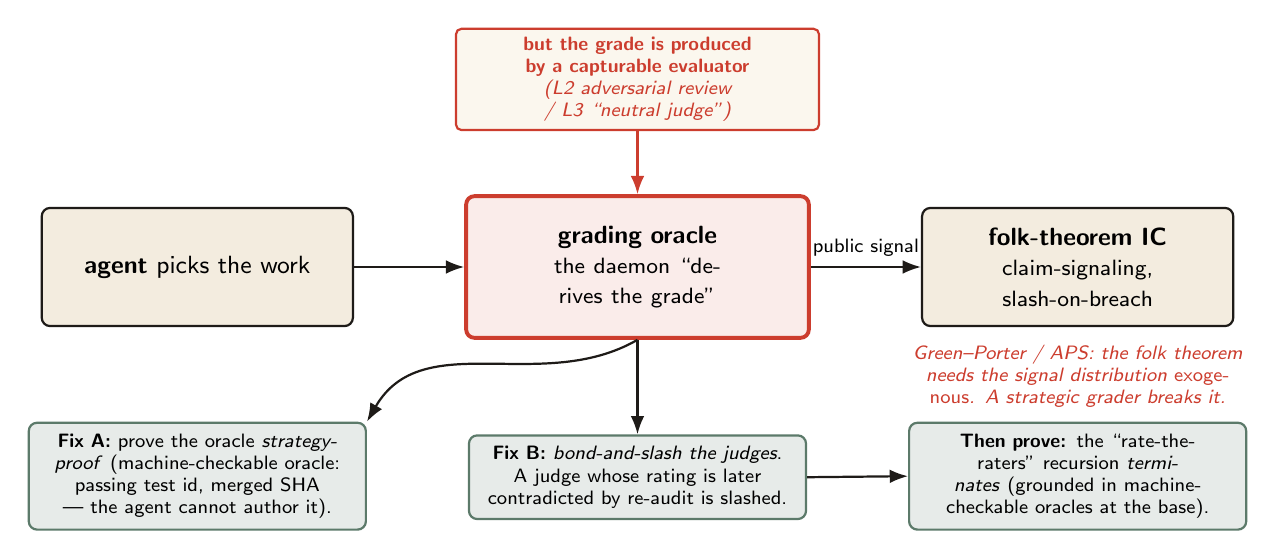
\begin{tikzpicture}[
  font=\sffamily\small,
  box/.style={draw=hhebony,thick,fill=hhsand!55,rounded corners=3pt,
              inner sep=5pt,text width=36mm,align=center,minimum height=15mm},
  oracle/.style={draw=hhcinnabar,line width=1.4pt,fill=hhcinnabar!10,
                 rounded corners=3pt,inner sep=5pt,text width=40mm,
                 align=center,minimum height=18mm},
  fix/.style={draw=hhpatina,thick,fill=hhpatina!15,rounded corners=3pt,
              inner sep=4pt,text width=40mm,align=center,font=\sffamily\scriptsize},
  flow/.style={->,>=Latex,thick,draw=hhebony},
]

% the folk-theorem chain
\node[box] (agent) at (0,0) {\textbf{agent} picks the work};
\node[oracle,right=14mm of agent] (grade) {\textbf{grading oracle}\\
  \footnotesize the daemon ``derives the grade''};
\node[box,right=14mm of grade] (folk) {\textbf{folk-theorem IC}\\
  \footnotesize claim-signaling, slash-on-breach};

\draw[flow] (agent) -- (grade);
\draw[flow] (grade) -- node[above,font=\sffamily\scriptsize]{public signal} (folk);

% the capture attack
\node[draw=hhcinnabar,thick,fill=hhpaper,rounded corners=2pt,inner sep=3pt,
      font=\sffamily\scriptsize\itshape,text=hhcinnabar,text width=44mm,
      align=center,above=8mm of grade] (capture)
  {\textbf{but the grade is produced by a capturable evaluator}\\
   (L2 adversarial review / L3 ``neutral judge'')};
\draw[->,>=Latex,thick,hhcinnabar] (capture) -- (grade);
\node[font=\sffamily\scriptsize\itshape,text=hhcinnabar,below=1mm of folk,
      text width=42mm,align=center]
  {Green--Porter / APS: the folk theorem needs the signal distribution
   \emph{exogenous}. A strategic grader breaks it.};

% the two fixes
\node[fix,below=12mm of agent] (sp)
  {\textbf{Fix A:} prove the oracle \emph{strategy-proof} (machine-checkable
   oracle: passing test id, merged SHA --- the agent cannot author it).};
\node[fix,below=12mm of grade] (bond)
  {\textbf{Fix B:} \emph{bond-and-slash the judges}. A judge whose rating is
   later contradicted by re-audit is slashed.};
\node[fix,below=12mm of folk] (rec)
  {\textbf{Then prove:} the ``rate-the-raters'' recursion \emph{terminates}
   (grounded in machine-checkable oracles at the base).};

\draw[flow] (grade.south) -- (bond.north);
\draw[flow] (bond.east) -- (rec.west);
\draw[flow] (grade.south) to[out=-150,in=60] (sp.north east);

\end{tikzpicture}%
}
\caption{The grading-oracle incentive-compatibility problem --- the hole under the
core theorem. Every folk-theorem claim in the layer bottoms out in ``the agent
picks the work, the daemon derives the grade.'' But a folk theorem is only as good
as the \emph{public signal} it conditions on (Green--Porter 1984;
Abreu--Pearce--Stacchetti 1990 require the signal distribution to be common
knowledge and \emph{exogenous}). The grade is produced by a capturable evaluator,
so the signal is endogenous and the folk theorem does not apply as stated. We
resolve it two ways: ground settlement in \emph{machine-checkable} oracles the
agent cannot author (Fix A, strategy-proof by construction), and \emph{bond-and-
slash} the human/LLM judges where machine-checking is impossible (Fix B), then
require the rate-the-raters recursion to terminate at a machine-checkable base.}
\label{fig:he-grading-oracle}
\end{figure}


\begin{theorem}[The folk theorem needs an exogenous signal]\label{thm:folk}
An imperfect-monitoring folk theorem (\textbf{Green--Porter}~1984; \textbf{Abreu--
Pearce--Stacchetti}~1990~\cite{aps1990}) requires the public-signal distribution to
be common knowledge and \emph{exogenous}. If the signal (the grade) is produced by a
strategic, capturable agent, the signal is endogenous and the folk theorem does not
apply as stated. The layer's deepest theorem sits on an un-modeled foundation unless
the oracle is made strategy-proof or the judges are bonded.
\end{theorem}

\noindent\textbf{The two resolutions (both used).}
\emph{Fix A --- strategy-proof by construction:} ground settlement in
\emph{machine-checkable} oracles the agent cannot author (a passing test id, a
merged SHA, a satisfied Arbiter check). Where this is possible, the oracle is
strategy-proof and Theorem~\ref{thm:folk}'s premise is met.
\emph{Fix B --- bond-and-slash the judges:} where machine-checking is impossible
(aesthetics, ambiguous quality), the human/LLM judges get their \emph{own} bond and
their \emph{own} reputation; a judge later contradicted by re-audit is slashed. The
``rate-the-raters'' recursion must then be shown to terminate at a machine-checkable
base, not regress infinitely. De-biasing for LLM judges (order-swap, pairwise,
family-exclude) follows \textbf{Zheng et al.}~2023~\cite{zheng2023}.

\begin{exercises}
\item State the exact assumption Theorem~\ref{thm:folk} needs about the public
  signal, and explain why a capturable grader violates it.
\item Classify three settlement criteria as machine-checkable (Fix A) or judge-
  dependent (Fix B): a unit test passing; a merged SHA; ``the refactor is
  tasteful.''
\item \openstar Prove the rate-the-raters recursion terminates: define a well-
  founded order on ``levels of judge,'' grounded at machine-checkable oracles, and
  show no infinite ascending chain of ``judges judging judges'' is needed.
\end{exercises}

% ═══════════════════════════════════════════════════════════════════════════════
\section{Hosted trust is the product (C3)}\label{sec:hosted-trust}
% ═══════════════════════════════════════════════════════════════════════════════

The 2025--26 agentic-payments landscape --- \textbf{AP2} (Google, signed payment
mandates), \textbf{ACP} (OpenAI/Stripe), and \textbf{x402} (Coinbase, stablecoin
settlement over HTTP) --- has commoditized the \emph{settlement rail}. Wiring an
agent to pay another agent is now table stakes. This is \emph{good news} for the
thesis, because it sharpens what the product actually is.

What remains scarce, and therefore defensible, is \textbf{hosted trust}: the
verified ledger (conservation-checked, Merkle-anchored evidence), the \emph{relay}
(the harbor mesh carrying public-key attestation across machines, ADR-0027), and the
\emph{reputation} that makes a counterparty you do not own legible and accountable.

\begin{itemize}[leftmargin=1.4em,itemsep=2pt]
  \item \textbf{Substrate (swappable):} the payment rail. Use x402/AP2/credits/
    Stripe interchangeably.
  \item \textbf{Product (the moat):} attestation, federation membership, and
    reputation hosting.
\end{itemize}

The revenue model aligns incentives without perverse over-penalty: a transaction
fee (2--5\% of settlements), a small listing fee (collusion deterrent), and a small
bond-spread on \emph{forfeited} bonds (kept small so the platform never profits from
over-slashing). The platform should earn most from \emph{successful} trade, because
successful trade is what hosted trust produces.

\pullquote{You don't sell crypto --- crypto is the substrate. The defensible asset
is attestation $+$ federation membership $+$ reputation, not the commoditized
payment rail.}

% ═══════════════════════════════════════════════════════════════════════════════
\section{Cold start, and the auction question}\label{sec:cold-start}
% ═══════════════════════════════════════════════════════════════════════════════

A three-sided market has a \emph{triple} cold-start problem: no operators shop an
empty fleet shelf; no owners list agents with no renters; no licensors publish
skills with no buyers. Two-sided-market theory prescribes: subsidize the side
carrying the scarcest cross-side externality, then flip. Phase~1 seeds supply at
zero/negative price with platform-posted tasks at above-market bounties (generating
the first settled outcomes --- the seed reputation data); Phase~2 imports external
work history for partial credit to break the new-agent freeze; Phase~3 flips to
charging the demand side once a liquidity threshold (not a calendar date) is met.

\subsection{Static escrow vs.\ competitive underwriting}\label{sec:fh-equilibria}\label{sec:youle:welfare}

% Static escrow vs Competitive Vickrey — placed inline near §sec:youle:welfare.
% Fragment intended for \input from the main paper; depends on tikz, hh* color
% definitions, and the styles defined in appendix-figures.tex (or this file
% redefines if loaded standalone).

\providecolor{hhsand}{HTML}{E9DCC4}
\providecolor{hhsanddeep}{HTML}{D4C5A9}
\providecolor{hhebony}{HTML}{1E1B18}
\providecolor{hhink}{HTML}{2C2A26}
\providecolor{hhcinnabar}{HTML}{CC3D2E}
\providecolor{hhbrass}{HTML}{B08D57}
\providecolor{hhpatina}{HTML}{5C7A6A}
\providecolor{hhpaper}{HTML}{FBF7EE}

\begin{figure}[H]
\centering
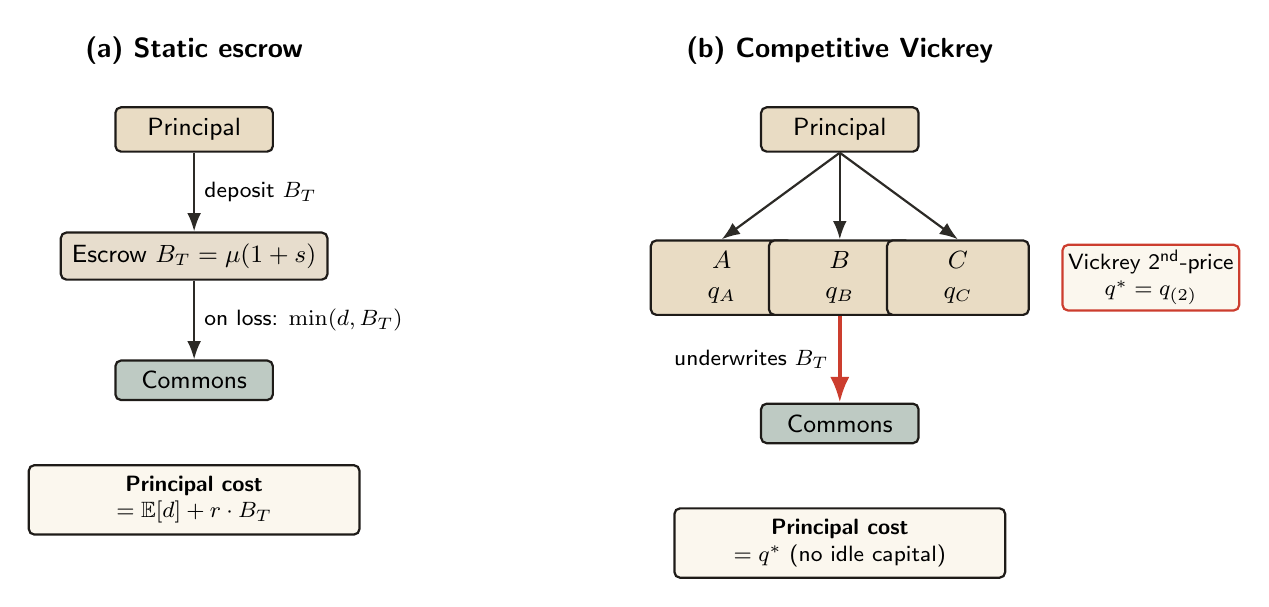
\begin{tikzpicture}[
  font=\sffamily\small,
  actor/.style={draw=hhebony,thick,fill=hhsand,rounded corners=2pt,
                inner sep=4pt,minimum width=20mm,align=center},
  commons/.style={draw=hhebony,thick,fill=hhpatina!40,rounded corners=2pt,
                  inner sep=4pt,minimum width=20mm,align=center},
  escrow/.style={draw=hhebony,thick,fill=hhbrass!30,rounded corners=2pt,
                 inner sep=4pt,minimum width=20mm,align=center},
  ins/.style={draw=hhebony,thick,fill=hhpaper,rounded corners=2pt,inner sep=4pt,
              align=center,minimum width=18mm},
  arr/.style={->,>=Latex,thick,draw=hhink},
]
\begin{scope}[xshift=0cm]
\node[font=\sffamily\bfseries,anchor=center] at (1.2,4.2) {(a) Static escrow};
\node[actor] (p1) at (1.2,3.2) {Principal};
\node[escrow,below=10mm of p1] (esc) {Escrow $B_T = \mu(1+s)$};
\node[commons,below=10mm of esc] (c1) {Commons};
\draw[arr] (p1.south) -- node[right,font=\sffamily\footnotesize]
  {deposit $B_T$} (esc.north);
\draw[arr] (esc.south) -- node[right,font=\sffamily\footnotesize]
  {on loss: $\min(d, B_T)$} (c1.north);
\node[align=center,font=\sffamily\footnotesize,
      draw=hhebony,thick,fill=hhpaper,rounded corners=2pt,inner sep=4pt,
      below=8mm of c1,minimum width=42mm] (cost1)
  {{\bfseries Principal cost} \\ $= \mathbb{E}[d] + r \cdot B_T$};
\end{scope}
\begin{scope}[xshift=8.2cm]
\node[font=\sffamily\bfseries,anchor=center] at (1.2,4.2)
  {(b) Competitive Vickrey};
\node[actor] (p2) at (1.2,3.2) {Principal};
\node[ins,fill=hhsand,below=11mm of p2,xshift=-15mm] (i1) {$A$\\$q_A$};
\node[ins,fill=hhsand,below=11mm of p2] (i2) {$B$\\$q_B$};
\node[ins,fill=hhsand,below=11mm of p2,xshift=15mm] (i3) {$C$\\$q_C$};
\node[commons,below=11mm of i2] (c2) {Commons};
\node[draw=hhcinnabar,thick,fill=hhpaper,rounded corners=2pt,inner sep=2pt,
      font=\sffamily\footnotesize,right=4mm of i3,align=center]
  (vic) {Vickrey 2\textsuperscript{nd}-price\\$q^* = q_{(2)}$};
\draw[arr] (p2.south) -- (i1.north);
\draw[arr] (p2.south) -- (i2.north);
\draw[arr] (p2.south) -- (i3.north);
\draw[arr,line width=1.4pt,draw=hhcinnabar] (i2.south) --
  node[left,font=\sffamily\footnotesize]
  {underwrites $B_T$} (c2.north);
\node[align=center,font=\sffamily\footnotesize,
      draw=hhebony,thick,fill=hhpaper,rounded corners=2pt,inner sep=4pt,
      below=8mm of c2,minimum width=42mm] (cost2)
  {{\bfseries Principal cost} \\ $= q^*$ (no idle capital)};
\end{scope}
\end{tikzpicture}
\caption{Static escrow vs.\ competitive Vickrey auction. Both regimes underwrite the same coverage $B_T = \mu(1+s)$; only the financing mechanism differs. In (a) the principal ties up $B_T$ for the coverage period, paying an opportunity cost $r \cdot B_T$. In (b) insurers compete; the principal pays only the second-lowest bid $q^*$. The competitive regime Pareto-dominates the static one under the welfare assumptions of \S\ref{sec:youle:welfare} below.}
\label{fig:auction-inline}
\end{figure}


Thomas Youle's competitive-insurance proposal --- insurer-agents bid to underwrite
transactions, replacing a static bond parameter with a market-discovered price --- is
a possible \emph{fourth} side. But it may collide with the Cleanup Lower Bound:

\begin{proposition}[Underwriting reframes the bond as reserve adequacy]\label{prop:reserve}
The Cleanup Lower Bound requires bond $\ge$ worst-case cleanup cost $c$. A
competitive insurance market prices to \emph{expected} loss, which sits below the
worst case for any below-tail agent. Either underwriting violates the Cleanup Lower
Bound (the commons can leak in the tail), or the bound must be reframed as the
\emph{insurer's} capital-adequacy constraint (a reserve-requirement framing with
tail reinsurance), not a per-transaction bond. The \emph{form} of the answer is
determined; only the reserve formula is open.
\end{proposition}

\subsection{Cartels and wash-trading}\label{sec:fh-failure-modes}\label{fig:cartel-folk}

% Figure IV.14 --- cartel stability is a two-lever phase diagram.
%
% Reader question: under which detection probabilities and sampled losses
% does collusion stop paying?
% Claim: the repeated-game boundary $V_C=\pi_D$ separates a region where
% deviation dominates from one where the discounted collusive stream still
% wins, and a rare severe loss can sit on the same boundary as a frequent
% smaller one.
% Evidence: $V_C=(\pi_C-p_dL)/(1-\delta(1-p_d))$, the two worked points
% (rare/severe; frequent/smaller) that this section marks on the boundary.
% Must distinguish: the two named regions (a verdict each) from the two
% specific worked points on the boundary between them.
% Grammar chosen: payoff inequality as a phase/regime plot (atlas first
% choice for IV/fig:cartel-game-inline). Grammar rejected: a decorative
% seesaw or five ticks with no scale (atlas reject list) -- neither carries
% the boundary's shape or the two worked points.
% Five-second test: a reader can find both worked points on the same
% boundary curve and say which region each one falls in.
\begin{figure}[H]
\centering
\pdfigurehue{pdgold}%
\begin{tikzpicture}[pd figure,x=1cm,y=1cm]
  \draw[pd rule,->] (-0.30,-1.45) -- (5.30,-1.45);
  \draw[pd rule,->] (-0.30,-1.45) -- (-0.30,3.15);
  \node[pd label,anchor=west] at (5.45,-1.45) {detection probability $p_d$};
  \node[pd label,rotate=90,anchor=south] at (-0.70,.80) {loss if detected $L$};
  % ---- the two regions, edged by the boundary they share -------------------
  \begin{scope}[on background layer]
    \fill[pd ready fill]
      (0.30,2.65) -- (1.70,2.00) -- (3.10,1.05) -- (3.95,.35) -- (4.50,-.15)
      -- (4.90,-.85) -- (4.90,3.15) -- (0.30,3.15) -- cycle;
    \fill[pd warn fill]
      (0.30,2.65) -- (1.70,2.00) -- (3.10,1.05) -- (3.95,.35) -- (4.50,-.15)
      -- (4.90,-.85) -- (4.90,-1.45) -- (0.30,-1.45) -- cycle;
  \end{scope}
  \draw[pd focus rule,line width=1.4pt]
    (0.30,2.65) -- (1.70,2.00) -- (3.10,1.05) -- (3.95,.35) -- (4.50,-.15)
    -- (4.90,-.85);
  \node[pd focus label,anchor=south west] at (0.45,2.72)
    {boundary $V_C=\pi_D$};
  \node[pd label,align=center,text width=2.5cm] at (3.60,2.55)
    {deviation pays\\cartel unstable};
  \node[pd label,align=center,text width=2.3cm] at (1.72,-.05)
    {collusion pays\\discounted stream wins};
  % ---- the two worked points, on the shared boundary ------------------------
  \node[pd datum] at (1.70,2.00) {};
  \node[pd tag,anchor=south east] at (1.53,2.10) {rare, severe};
  \node[pd datum] at (3.95,.35) {};
  \node[pd tag,anchor=north east] at (3.78,.20) {frequent, smaller};
\end{tikzpicture}
\caption{\textbf{Cartel sustainability in the detection--loss plane.} The
curve marks $V_C=\pi_D$: below it collusion pays; above it deviation pays.
The two marked policies share the boundary, so detection frequency alone does
not determine stability. [internal]}
\label{fig:cartel-game-inline}
\end{figure}


Multi-homing plus portable reputation enables cross-harbor \emph{cartels} (a rating
cartel is the closest real-world analogue to ``the harbor's universities and rating
agencies''). And a colluding requester$+$worker can \emph{wash-trade} fake settled
outcomes to mint reputation cheaply. The defense form --- cost-per-settled-outcome
must exceed reputation's marginal value --- is circular as stated, because that
marginal value is endogenous to the same market. The fix is a structural break:
make settled outcomes between a counterparty \emph{pair} exhibit sharply diminishing
reputation returns (a concavity that caps the wash-trade payoff regardless of
price), plus sampled adversarial re-audit of high-velocity pairs.

\begin{exercises}
\item Which side should Phase~1 subsidize, and why? Apply the ``scarcest cross-side
  externality'' rule.
\item Use Figure~\ref{fig:cartel-game-inline} to identify the grim-trigger
  condition under which the cartel is self-sustaining. What raises the critical
  discount factor $\delta$ enough to break it?
\item \openstar ``Price of anarchy when reputation is for sale'' is the wrong tool:
  once reputation is tradeable, you have changed the game, so PoA (a ratio for a
  \emph{fixed} game) does not apply. Reframe it as a \emph{signal-existence}
  question (Spence-signaling with a resale market): does \emph{any} informative
  separating equilibrium survive reputation resale?
\end{exercises}

% ═══════════════════════════════════════════════════════════════════════════════
\section{The sheaf-gluing problem (one question, three guises)}\label{sec:sheaf}
% ═══════════════════════════════════════════════════════════════════════════════

Three of the layer's open problems --- trustless cross-harbor settlement, the
equivocation/convergence race, and the cross-harbor unit-of-account --- are the
\emph{same} problem in different clothes.

\begin{conjecture}[The gluing obstruction]\label{conj:sheaf}
Consider the assignment $\textsf{harbor}\mapsto\textsf{its ledger}$. Federation
succeeds iff this assignment forms a \emph{sheaf}: local sections (per-harbor
ledgers) glue to a unique global section (federated state) exactly when they agree
on overlaps (cross-harbor conservation). The double-spend / equivocation race is the
\emph{non-vanishing of the first cohomology $H^1$ of the gluing} --- the precise
obstruction to gluing local-consistent ledgers into one global-consistent state.
Open Problems on settlement (Conj.~\ref{conj:trustless}), equivocation
(Conj.~\ref{conj:eq-bound}), and unit-of-account
(Theorem~\ref{thm:lax}) are this single obstruction. (\Open{}.)
\end{conjecture}

This earns the Spivak/applied-category-theory citation honestly rather than
decoratively (\textbf{Fong \& Spivak}, \emph{Seven Sketches in
Compositionality}~\cite{fong2019}): it sharpens three vague problems into one precise
one and tells a defense exactly what it must kill --- the $H^1$ class.

\begin{exercises}
\item In one sentence each, restate Conjectures~\ref{conj:trustless},
  \ref{conj:eq-bound}, and Theorem~\ref{thm:lax} as facets of the gluing
  obstruction.
\item Why is double-spend ``$H^1 \ne 0$'' and not ``$H^0 \ne 0$''? (Hint: $H^0$ is
  global sections; $H^1$ is the obstruction to building one.)
\item \openstar Either exhibit a defense that forces $H^1 = 0$ for a bounded gossip
  topology, or prove no such defense exists without consensus (which would refute
  the federation thesis's no-consensus stance).
\end{exercises}

% ═══════════════════════════════════════════════════════════════════════════════
\section{Gaps the design must still close}\label{sec:gaps}
% ═══════════════════════════════════════════════════════════════════════════════

Honesty requires naming what is unspecified. These are not threats already
defended; they are holes.

\begin{enumerate}[leftmargin=1.6em,itemsep=3pt]
  \item \textbf{Multi-dimensional reputation aggregation.} ``Accuracy/aesthetics/
    efficiency judged by separate experts'' has no specified combination rule.
    Categorically, it is a functor into a product object with no chosen universal
    map to $\mathbb{R}$; you cannot have ``separate axes'' and ``one buyer-readable
    score'' without specifying the cone. (\Vision{}.)
  \item \textbf{Float-plan amendment under scope drift.} The four states assume the
    acceptance criteria were right. Mid-flight re-specification needs a re-sign
    protocol with escrow top-up/refund delta, preserving conservation.
  \item \textbf{Cross-boundary key rotation.} How a rotated signing key
    invalidates or re-validates cross-harbor delegations already held by $B$ is
    unspecified.
  \item \textbf{Skill versioning.} Reputation attaches to a content hash; v2 starts
    cold. The lemons problem reappears at every version bump.
  \item \textbf{Operator exit / harbor death.} Escrow orphaning, in-flight float
    plans, and reputation tombstoning on ungraceful exit are unspecified --- the L3
    analogue of the L0 resurrection problem.
  \item \textbf{Incentive-compatible arbitration capacity.} The human oracle is
    scarce and expensive; at scale arbitration is itself a priced, bondable,
    slashable service that must converge to honest rulings, not rubber-stamping.
\end{enumerate}

% ═══════════════════════════════════════════════════════════════════════════════
\section{Honest state of the layer}\label{sec:honest}\label{app:fh-mech}
% ═══════════════════════════════════════════════════════════════════════════════

\begin{table}[H]
\centering
\small
\caption{Per-claim honest state, consistent with shipped code and the ADRs
(ADR-0045 discipline). The one-line summary: a \Built{} conserving bond ledger, a
\Built{} continuity organ (memory), a \BuiltWeak{} checkpoint, and a richly
\Designed{}-and-model-verified protocol stack --- but the spine the market trades on
(non-forgeable cross-operator identity $\to$ outcome ledger $\to$ reputation) is
\Designed{}-to-\Vision{}. Today the harbor economy is a two-sided market with a
proof-backed roadmap to three.}
\label{tab:honest-state}
\begin{tabular}{@{}p{7.6cm} l p{4.4cm}@{}}
\toprule
\textbf{Claim / mechanism} & \textbf{State} & \textbf{Grounding} \\
\midrule
Bond ledger: escrow, slash, commons pool & \Built{} & \texttt{lib/bonds.ts} \\
Conservation $\text{wallet}+\text{escrow}+\text{commons}=\text{supply}$ & \Built{} &
  10k-trace property test \\
No-spawn-without-bond & \BuiltWeak{} & escrow-first; runtime gate is Phase-2 \\
Episodic memory (continuity organ 1) & \Built{} & \texttt{lib/episodic-memory.ts} \\
Resurrection / checkpoint (organ 2) & \BuiltWeak{} & passes notes, not state \\
Outcome ledger (organ 3 --- reputation keys here) & \Designed{} &
  ADR-0041, \texttt{lib/commitments.ts} \\
Non-forgeable actor identity (intra-harbor) & \Designed{} & ADR-0040 \\
Cross-operator attestation & \Designed{}/\Vision{} & ADR-0040b (unwritten) \\
Float plan $+$ \texttt{ed25519} escrow ceremony & \Designed{} & ADR-0014 \\
Anchor capability transfer (attenuation) & \Designed{} & verified \emph{as model} \\
Reputation estimator (Elo/BT/TrueSkill) & \Designed{}/\Vision{} & no \texttt{lib/reputation.ts} \\
Multi-dimensional reputation, neutral judges & \Vision{} & no axis-aggregation spec \\
Three-sided market (labor/rental/licensing) & \Designed{} & two-sided in reality \\
Skill licensing (metered $+$ clawback $+$ Merkle proof) & \Designed{} &
  cross-harbor verifiability undeployed \\
Federation: witness log, capability transfer & \Designed{} & federated-harbor paper \\
Bounded escrow (extraction $\le \varphi$) & \Designed{} (theorem) & trustless variant conjectured impossible \\
Cross-harbor conservation & \Designed{} (property) & \texttt{fh-cross-cons} $+$ TLA\textsuperscript{+} \\
Federated revocation convergence & \Designed{} (theorem) & equivocation race \Open{} \\
Hosted-trust moat / rail separation & \Designed{} (positioning) & not a code artifact \\
Competitive underwriting (Youle, 4th side) & \Vision{} & composition unresolved \\
\bottomrule
\end{tabular}
\end{table}

% ═══════════════════════════════════════════════════════════════════════════════
\section{Conclusion}\label{sec:conclusion}
% ═══════════════════════════════════════════════════════════════════════════════

The harbor-master makes a swarm legible, accountable, and safe for one operator (the
wedge of Paper~1). When operators sail out to trade, the \emph{same} ledger that
kept one operator's swarm honest becomes the market that lets fleets who don't trust
each other work together: three sides, one bond, hosted trust. We have not papered
over the cost of that claim. The keystone identity ADR covers a single-operator
threat model and must be extended to ADR-0040b before the boundary is honestly one
``neither controls.'' Conservation composes upward only as a functor within a single
unit of account, and a $\varphi$-bounded lax functor otherwise. Reputation is
monotone in honest outcomes and revocable by tombstone, not by Sagas. Every folk-
theorem result rests on a grading oracle that must be machine-checkable or bonded.
And strict conservation is budget balance, so by Myerson--Satterthwaite the market
gives up efficiency. The bones are good and the floor is built; the spine the market
trades on is designed, not shipped --- and this paper says so in the same words
throughout, because a market built on an overstated keystone is a market built on
sand.

% ═══════════════════════════════════════════════════════════════════════════════
\begin{thebibliography}{99}
% ═══════════════════════════════════════════════════════════════════════════════

\bibitem{rochet2003} J.-C. Rochet \& J. Tirole. ``Platform Competition in Two-Sided
Markets.'' \emph{Journal of the European Economic Association} 1(4):990--1029, 2003.

\bibitem{rochet2006} J.-C. Rochet \& J. Tirole. ``Two-Sided Markets: A Progress
Report.'' \emph{RAND Journal of Economics} 37(3):645--667, 2006.

\bibitem{armstrong2006} M. Armstrong. ``Competition in Two-Sided Markets.''
\emph{RAND Journal of Economics} 37(3):668--691, 2006.

\bibitem{grossman1986} S. Grossman \& O. Hart. ``The Costs and Benefits of
Ownership: A Theory of Vertical and Lateral Integration.'' \emph{Journal of
Political Economy} 94(4):691--719, 1986.

\bibitem{akerlof1970} G. Akerlof. ``The Market for `Lemons': Quality Uncertainty and
the Market Mechanism.'' \emph{Quarterly Journal of Economics} 84(3):488--500, 1970.

\bibitem{myerson1981} R. Myerson. ``Optimal Auction Design.'' \emph{Mathematics of
Operations Research} 6(1):58--73, 1981.

\bibitem{myerson1983} R. Myerson \& M. Satterthwaite. ``Efficient Mechanisms for
Bilateral Trading.'' \emph{Journal of Economic Theory} 29(2):265--281, 1983.

\bibitem{aps1990} D. Abreu, D. Pearce \& E. Stacchetti. ``Toward a Theory of
Discounted Repeated Games with Imperfect Monitoring.'' \emph{Econometrica}
58(5):1041--1063, 1990. (With Green \& Porter, \emph{Econometrica} 1984.)

\bibitem{liu2014} Q. Liu \& A. Skrzypacz. ``Limited Records and Reputation
Bubbles.'' \emph{Journal of Economic Theory} 151:2--29, 2014.

\bibitem{chiu2025} C. Chiu, S. Zhang \& M. van der Schaar. ``Strategic
Self-Improvement for Competitive Agents in AI Labour Markets.'' arXiv:2512.04988,
2025.

\bibitem{resnick2006} P. Resnick, R. Zeckhauser, J. Swanson \& K. Lockwood. ``The
Value of Reputation on eBay: A Controlled Experiment.'' \emph{Experimental
Economics} 9(2):79--101, 2006.

\bibitem{tadelis2016} S. Tadelis. ``Reputation and Feedback Systems in Online
Platform Markets.'' \emph{Annual Review of Economics} 8:321--340, 2016.

\bibitem{zheng2023} L. Zheng et al. ``Judging LLM-as-a-Judge with MT-Bench and
Chatbot Arena.'' \emph{NeurIPS} 2023.

\bibitem{douceur2002} J. Douceur. ``The Sybil Attack.'' \emph{IPTPS} 2002.

\bibitem{flp1985} M. Fischer, N. Lynch \& M. Paterson. ``Impossibility of
Distributed Consensus with One Faulty Process.'' \emph{Journal of the ACM}
32(2):374--382, 1985.

\bibitem{dls1988} C. Dwork, N. Lynch \& L. Stockmeyer. ``Consensus in the Presence
of Partial Synchrony.'' \emph{Journal of the ACM} 35(2):288--323, 1988.

\bibitem{laurie2014} B. Laurie. ``Certificate Transparency.'' \emph{Communications
of the ACM} 57(10):40--46, 2014.

\bibitem{laurie2013ct} B. Laurie, A. Langley \& E. Kasper. ``Certificate
Transparency.'' RFC 6962, IETF, 2013.

\bibitem{demers1987} A. Demers et al. ``Epidemic Algorithms for Replicated Database
Maintenance.'' \emph{PODC} 1987.

\bibitem{heilman2015} E. Heilman, A. Kendler, A. Zohar \& S. Goldberg. ``Eclipse
Attacks on Bitcoin's Peer-to-Peer Network.'' \emph{USENIX Security} 2015.

\bibitem{herlihy2018} M. Herlihy. ``Atomic Cross-Chain Swaps.'' \emph{PODC} 2018.

\bibitem{hls2022} M. Herlihy, B. Liskov \& L. Shrira. ``Cross-Chain Deals and
Adversarial Commerce.'' \emph{The VLDB Journal} 31:1291--1309, 2022.

\bibitem{sagas1987} H. Garcia-Molina \& K. Salem. ``Sagas.'' \emph{ACM SIGMOD} 1987.

\bibitem{spivak2012} D. Spivak \& R. Kent. ``Ologs: A Categorical Framework for
Knowledge Representation.'' \emph{PLoS ONE} 7(1):e24274, 2012.

\bibitem{fong2019} B. Fong \& D. Spivak. \emph{Seven Sketches in Compositionality:
An Invitation to Applied Category Theory.} Cambridge University Press, 2019.

\bibitem{ostrom1990} E. Ostrom. \emph{Governing the Commons.} Cambridge University
Press, 1990.

\bibitem{nrtv2007} N. Nisan, T. Roughgarden, É. Tardos \& V. Vazirani (eds.).
\emph{Algorithmic Game Theory.} Cambridge University Press, 2007.

\end{thebibliography}

\end{document}
